Autopilot je sistem sa zatvorenom povratnom spregom unutar sistema za vođenje objekta 
u prostoru koji osigurava da projektil dostigne ubrzanje koje mu sistem vođenja zapovjeda. 
Funkcija autopilota je da stabilizuje i vodi projektil tako što zadaje upravljačke signale kontrolnim 
površinama koji tjeraju projektil da se rotira odnosno da translira.  
Pošto tranzijentni odziv projektila varira sa promjenom uslova leta, tako i parametri 
autopilota treba da se mjenjaju sa uslovima leta pa prema tome dobro 
dizajniran autopilot osigurava skoro linearan odziv. Najčešće se za projektovanje 
autopilota koristi linearizirani model drugog reda koji je ranije izveden. 
Kada se radi o proporcionalnoj navigaciji, generišu se tri komponente ubrzanja koje projektil mora 
zadovoljiti kako bi osigurao susret sa metom. U nastavku su prikazani regulatori koji 
treba da osiguraju da projektil postigne zadata ubrzanja. Važno je samo istaći 
da su ubrzanja koja zadaje proporcionalna navigacija data u inercijalnom koordinatnom sistemu. Praksa 
je da se kao kontrolisane veličine koriste ubrzanja koja su normalna na vektor brzine. Prema tome, 
radi se o dvije komponente ubrzanja- \textit{horizontalno i vertikalno ubrzanje}. Vektor horizontalnog ubrzanje 
leži u $xy$ ravni inercijalnog koordinatnog sistema, a vektor vertikalnog ubrzanja leži u $xz$ ravnini inercijalnog
koordinatnog sistema. Kada projektil postigne zadata ubrzanja, on pravi kružne lukove u vertikalnoj i 
horizontaloj ravnini. Kako bi se načinila razlika između horizontalne i vertikalne ravni, potrebno je 
da se projektil ne valja oko svoje $x$ ose. Ovo ima još jedan pozitivan efekat jer se tada poništava 
sprega između kanala visine i kanala pravca. Dakle, za vođenje proporcionalnom 
navigacijom potrebna su tri regualtora:
\begin{itemize}
    \item Regulator vertikalnog ubrzanja(kanal visine)
    \item Regulator horizontalnog ubrzanja(kanal pravca)
    \item Regulator za stabiliaziciju valjanja(kanal valjanja)
\end{itemize}
Ova tri regulatora zajedno se zovu \textbf{autopilot}. 
U nastavku je predstavljen regulator za stabiliaziciju ugla propinjanaja te tri regualatora potrebna 
za realizaciju proporcionalne navigacije. 
\section{Upravljanje i stabilizacija ugla propinjanja}
Glavni zadatak autopilota ugla propinjanja je da stabilizuje projektil, tj. da 
pruži stabilizaciju propinjanja projektila oko longitudinalne ose. Ovo se postiže tako 
što se mjeri brzina propinjnnja i taj signal se koristi da bi se otklonile 
kontrolne površine za iznos koji je potreban da bi se borilo protiv poremećaja. 
Poremećaji u uglu propinjanja mogu nastati zbog atmosferskih porejemćaja ili 
zbog asimetričnosti letjelice. Dalje, često se zahtjeva da ugao propinjanja prati 
određenu referentnu vrijednost. Ovo se može zahtjevati kod "zemlja- zrak" projektila 
kod kojih se zahtjeva da projektil ima isti ugao pri kojem je lansiran sa platforme. 
Viđeno je ranije da odziv ugla propinjanja neograničeno raste na stalan otklon krmila visine 
i da u početku leta ima kratkoperiodične oscilacije. Uvođenjem povratne sprege,
može se postići da ugao propinjanja postigne zadatu stacionarnu vrijednost, ali kratkoperiodične 
oscilacije će i dalje ostati i mogu praviti probleme. Kratkoperiodične 
oscilacije se mogu ukloniti uvođenjem dodatne povratne sprege po brzini ugla propinjanja 
i time povećati stabilnost procesa. Uvođenjem integralnog kompenzatora može se povećati brzina odziva.
U nastavku će se projektovati regulator ugla propinjanja za linerizirani model longitudinalnog kretanja 
koji je dat prenosnom funkcijom:
\begin{equation}
    \frac{\Delta \theta(s)}{\Delta \delta_V(s)}=\frac{K(T_1s+1)}{s(T^2s^2+2\xi Ts+1)}
\end{equation}
Za $K=0.75$, $T_1 = 1s$, $\omega _n = 20 \frac{rad}{s}$ i $\xi = 0.1$. 
Postojanje nule u prenosnoj funkciji uvodi oscilacije i povećava preskok sistema sa 
zatvorenom povratnom spregom. Odziv ugla propinjanja na odskočnu pobudu  je dat na 
slici \ref{fig:propinj}
\begin{figure}[!ht]
    \centering
    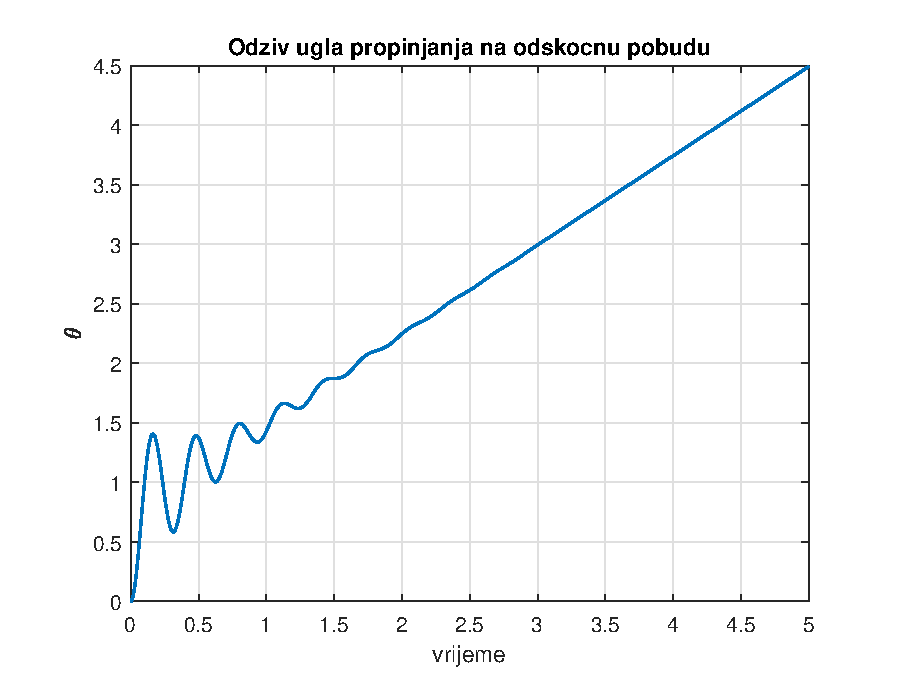
\includegraphics[scale = 0.7]{thetaOtvSprega.eps}
    \caption{Oodziv ugla propinjanja u otvorenoj povratnoj sprezi}
    \label{fig:propinj}
\end{figure} 
Ako se želi da ugao propinjanja prati neku referentnu vrijednost može se uvesti 
povratna sprega po uglu propinjanja preko slobodnog brzinskog žiroskopa. Blok dijagram sistem sa zatvorenom 
povratnom spregom po uglu propinjanja dat je na slici \ref{fig:slobGyro}.
 \begin{figure}[!ht]
     \centering
     \begin{tikzpicture}[auto, node distance=2cm,>=latex']
       \node[input, name=input](input){};
       \node[sum, right of = input](sum){};
       \node[block, right of = sum] (g1){$\frac{K(T_1s+1)}{T^2s^2+2\xi Ts+1}$};
       \node[block, right of = g1,node distance = 2.5cm] (g2){$\frac{1}{s}$};
       \node [output, right of = g2] (output) {};
       \node[block, below of = g1] (gyro){$K_G$};
       \draw [->] (g2) -- node [name=y, anchor = south] {$\theta$}(output);
       \draw[->] (y)|-(gyro);
       \draw[->] (gyro) -|node[pos=0.99] {$-$}(sum);
       \draw[->](g1) -- (g2);
       \draw [draw,->] (input) -- node {$u$} node[pos=0.99] {$+$}(sum);
       \node[anchor = south] (thetadot) at ($(g1)!0.6!(g2)$){$\dot{\theta}$};
       \draw[->] (sum)--(g1);
\end{tikzpicture}
\caption{Povratna sprega po uglu propinjanja}
\label{fig:slobGyro}
\end{figure}
Prenosna funkcija sistema sa zatvorenom povratnom spregom je data sa:
\begin{equation}
    \frac{\theta (s)}{\delta _V(s)} = \frac{\frac{K_GK(T_1s+1)}{T^2s^2+2\xi Ts+)}}{1+\frac{K_GK(T_1s+1)}{T^2s^2+2\xi Ts+)}}
    =\frac{K(T_1s+1)}{T^2s^3+2\xi Ts^2+(1+KK_GT_1)s+KK_G}
\end{equation}
Sada se vidi da je stacionarna vrijednost odziva ugla propinjanja na odskočnu pobudu:
\begin{equation}
    \theta _{stac} = \lim_{s \to 0} s\frac{1}{s}\frac{K(T_1s+1)}{T^2s^3+2\xi Ts^2+(1+KK_GT_1)s+KK_G} = \frac{1}{K_G}
\end{equation}

\begin{figure}[!ht]
    \centering 
    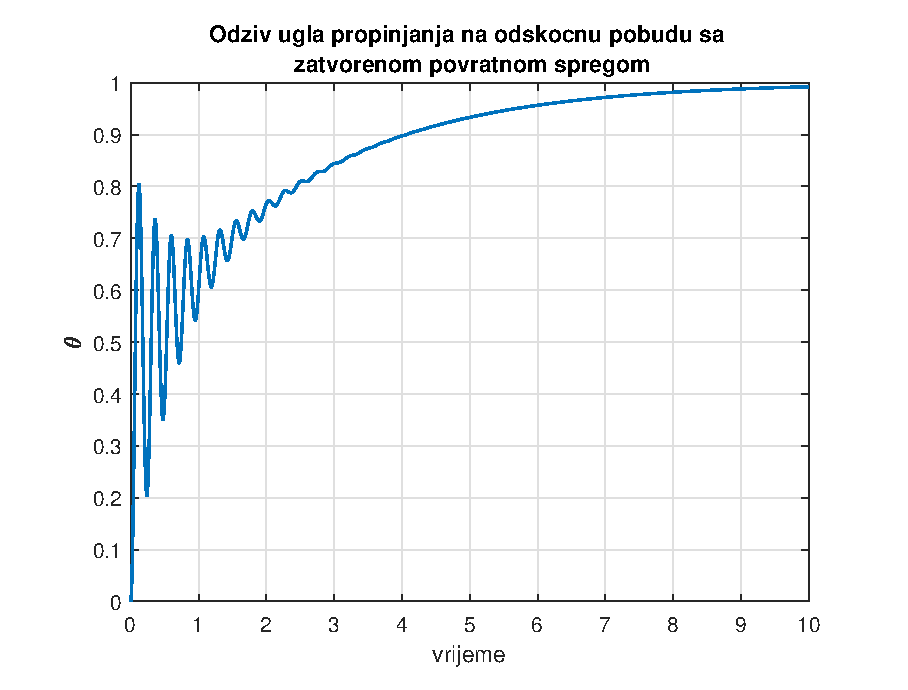
\includegraphics[scale = 0.7]{closedLoopPitch.eps}
    \caption{Odziv ugla propinjanja sa zatvorenom povratnom spregom po uglu propinjanja}
    \label{fig:closedPitch}
\end{figure}
Odziv ugla propinjanja sa zatvorenom povratnom spregom po uglu propinjanja je data na slici \ref{fig:closedPitch}
Sada se vidi da se uvođenjem povratne sprege po uglu propinjnja osigurava da ugao propinjanja prati referentnu 
vrijednost, ali se vidi i da je odziv sporiji  i da i dalje postoje kratkoperiodične oscilacije na početku propinjnanja.
Ove oscilacije su posljedica postojanja nule u prenostnoj funkciji zatvorene petlje. 
Uvođenjem integralnog kompenzatora, ova nula se može pokratiti sa polom kompenzatora i tako dobiti glađi odziv.
Uvedimo kompenzator sa prenosnom funkcijom:
\begin{equation}
    G_c(s) = \frac{\alpha T_cs+1}{T_cs+1}  \quad \alpha<1
\end{equation}
Ako se za pol kompenzatora uzme $T_c = T_1$, tada će nula sistema sa otvorenom 
povratnom spregom biti u $-\frac{1}{\alpha T_1}$ što daje veću kontrolu nad postavljanjem 
polova. Povoljnim odabirom parametra $\alpha$ nula se može postaviti na proivoljnu lokaciju.
Odziv sistema sa integralnim kompenzatorom je prikazan na slici \ref{fig:komp}.
\begin{figure}[!ht]
    \centering
    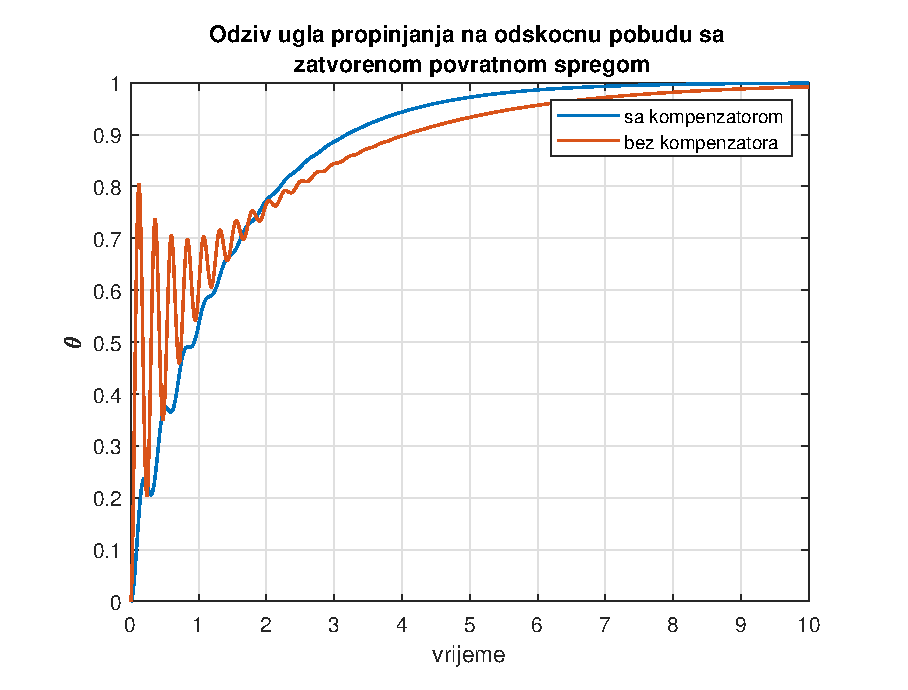
\includegraphics[scale = 0.5]{compareLead.eps}
    \caption{Odziv ugla propinjanja sa integralnim kompenzatorom}
    \label{fig:komp}
\end{figure}
Simulink blok dijagram za simulaciju odziva sa integralnim kompenzatorom je prikazan na 
slici \ref{fig:leadSim}
\begin{figure}[!ht]
    \centering
    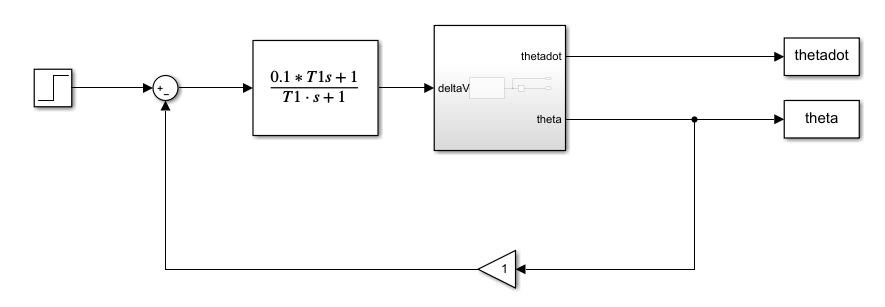
\includegraphics[scale = 0.5]{leadInteSim.JPG}
    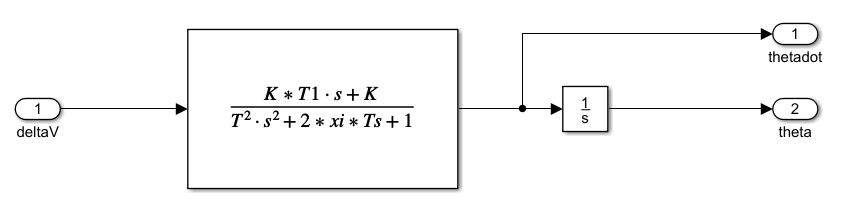
\includegraphics[scale= 0.5]{subKask.JPG}
    \caption{Regulacija sa integralnim kompenzatorom}
    \label{fig:leadSim}
\end{figure}
Dodatno, stabilnost odziva se može povećati uvođenjem dodatne povratne sprege po brzini 
ugla propinjanja. Ako se uvede povratna samo po brzini, tada će se stabilizovati samo 
brzina promjene ugla propinjanja a sam ugao propinjanja će imati oblik rampe. 
Blok dijagram ovog upravljačkog sistema je dat na slici \ref{fig:kask}.
\begin{figure}[!ht]
    \centering
    \begin{tikzpicture}[auto, node distance=2cm,>=latex']
        \node[input, name=input](input){};
       \node[sum, right of = input](sum2){};
       \node[sum, right of = sum2](sum){};
       \node[block, right of = sum] (g1){$\frac{K(T_1s+1)}{T^2s^2+2\xi Ts+)}$};
       \node[block, right of = g1,node distance = 2.5cm] (g2){$\frac{1}{s}$};
       \node [output, right of = g2] (output) {};
       \node[block, below of = g1] (gyrosA){$K_{GB}$};
       \node[block, below of = gyrosA, node distance = 1.5cm] (gyro){$K_{GA}$};
       \draw [->] (g2) -- node [name=y, anchor = south] {$\theta$}(output);
       \draw[->] (y)|-(gyro);
       \draw[->] (gyro) -|node[pos=0.99] {$-$}(sum2);
       \draw[->](g1) -- (g2);
       \draw [draw,->] (input) -- node {$u$} node[pos=0.99] {$+$}(sum2);
       \node[anchor = south] (thetadot) at ($(g1)!0.6!(g2)$){$\dot{\theta}$};
       \draw[->] (sum)--(g1);
       \draw[->] (sum2) -- node[pos = 0.99]{$+$}(sum);
       \draw[->] (gyrosA)-| node[pos = 0.99] {$-$}(sum);
       \draw[->] (thetadot)|-(gyrosA);
\end{tikzpicture}
\caption{Povratna sprega po brzini i uglu propinjanja}
\label{fig:kask}
\end{figure}
Vrijednost izvoda ugla propinjanja se dobija pomoću brzinkskog žiroskopa, a 
vrijednost ugla propinjanja se dobija pomoću slobodnog žiroskopa. Pojačanje povratne 
grane iznosi:
\begin{equation}
    H(s)=K_{GA}+sK_{GB}
\end{equation}
,a pojačanje direktne grane je:
\begin{equation}
    P(s)=\frac{1}{s}\frac{K(T_1s+1)}{T^2s^2+2\xi Ts+)}
\end{equation}
Pa je ukupna funkcija prenosa:
\begin{equation}
    \frac{\theta(s)}{\delta _V(s)} = \frac{K(T_1s+1)}{T^2s^3+
    (2\xi T+KK_{GB}T_1)s^2+(1+KK_{GB}+KK_{GA}T_1)s+KK_{GA}}
\end{equation}
Ovaj sistem je prikazan Simulink blok dijagramom na slici \ref{fig:simuKask}.
\begin{figure}[!ht]
    \centering
    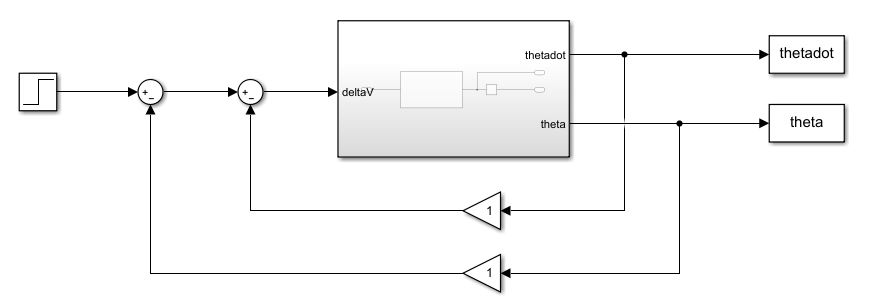
\includegraphics[scale = 0.5]{simKask.JPG}
    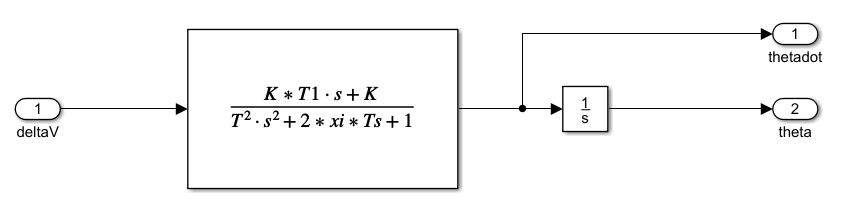
\includegraphics[scale = 0.5]{subKask.JPG}
    \caption{Simulink shema kaskadne regulacije ugla propinjanja}
    \label{fig:simuKask}
\end{figure}
Stacionarna vrijednost na odskočnu pobudu iznosi $\frac{1}{K_{GA}}$
\begin{figure}[!ht]
    \centering
    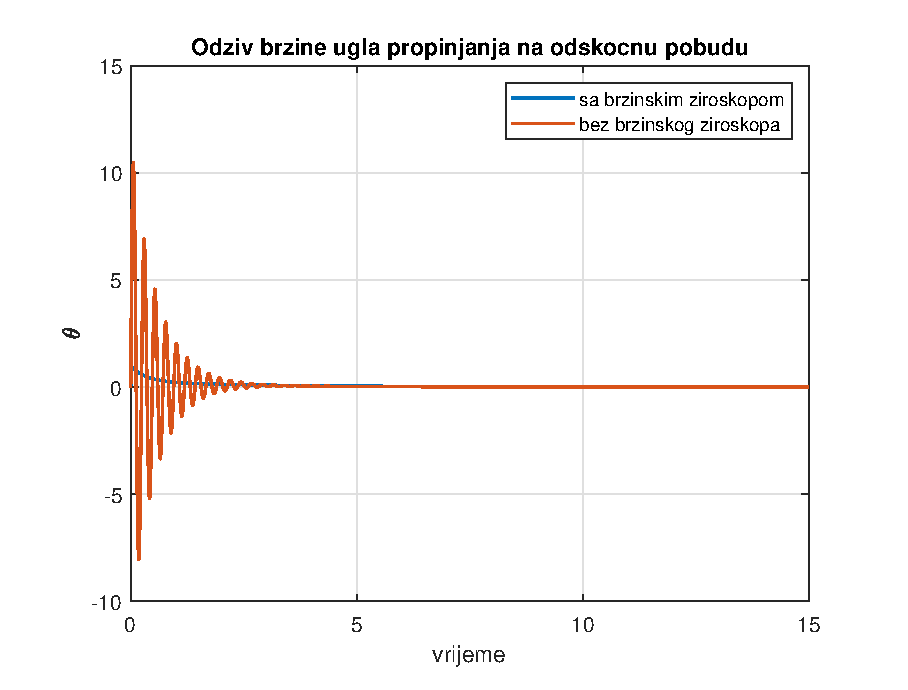
\includegraphics[scale = 0.5]{poredjenjeBrzina.eps}
    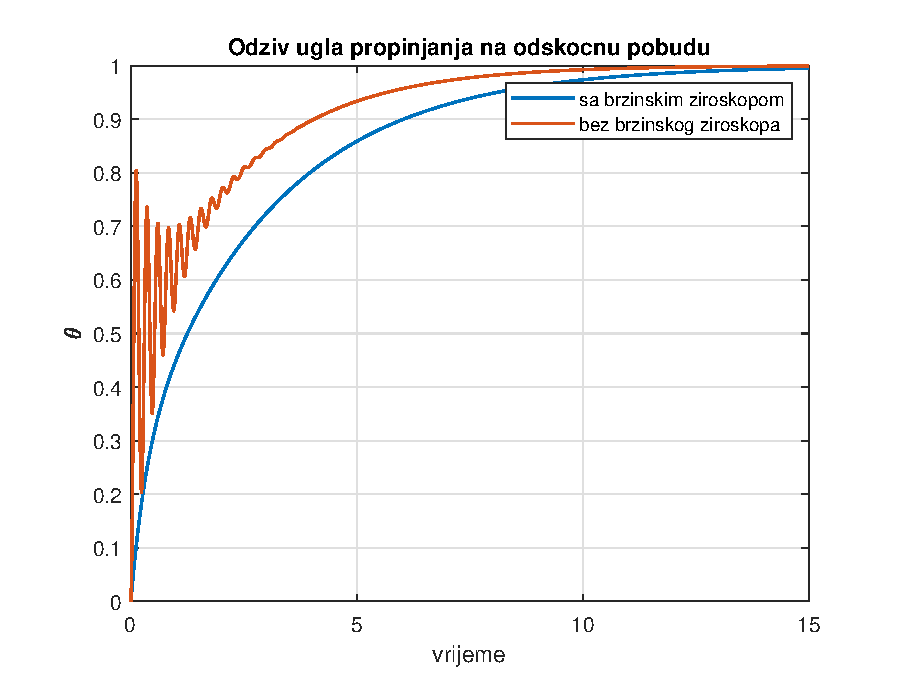
\includegraphics[scale = 0.5]{poredjenjeOdziva.eps}
    \caption{Odzivi ugla propinjanja sa povratnom spregom po brzini i uglu propinjanja}
\end{figure}
%\begin{figure}[!ht]
%    \centering
%    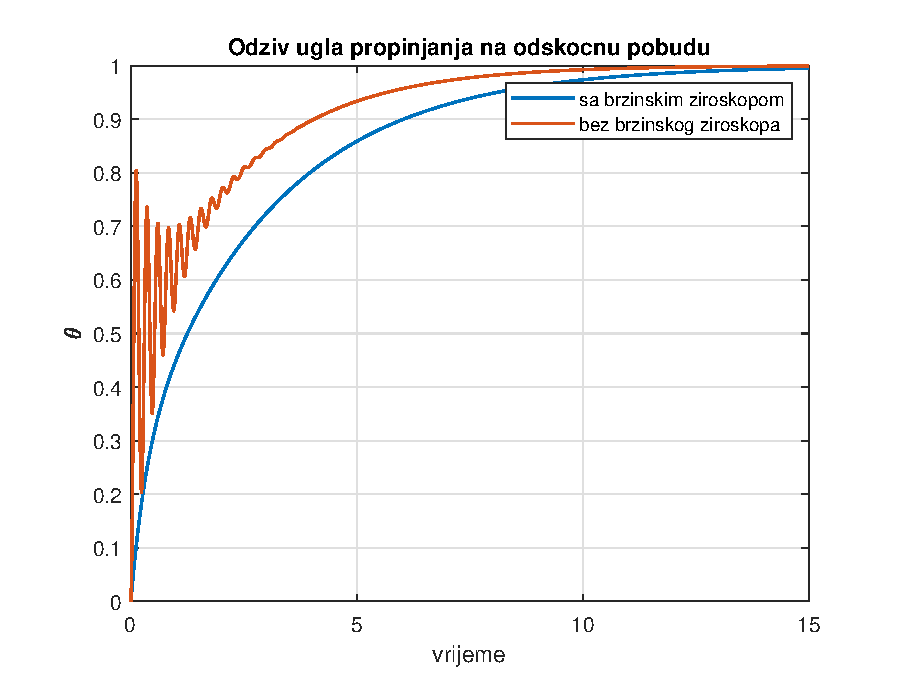
\includegraphics{poredjenjeOdziva.eps}
%\end{figure}
\section{Upravljanje vertikalnim ubrzanjem}
Kako je razmatrano u prethodnom poglavlju, kod proporcionalne navigacije, se projektilu 
zadaju normalna ubrzanja kako bi on pogodio metu pa je od posebnog interesa imati sistem 
za regulaciju normalnog ubrzanja projektila. Jasno je da će to opet biti upravljanje u 
zatvorenoj povratnoj sprezi. Normalno ubrzanje projektila pri longitudinalnom kretanju 
je dato prenosnom funkcijom:
\begin{equation}
    \frac{n_L(s)}{\delta_V(s)}=\frac{KV}{T^2s^2+2\xi Ts+1}
\end{equation}
Stacionarna vrijednost iznosi $KV$. Odziv na odskočni otklon krmila visine je dat 
na slici \ref{fig:nLodziv}
\begin{figure}[!ht]
    \centering
    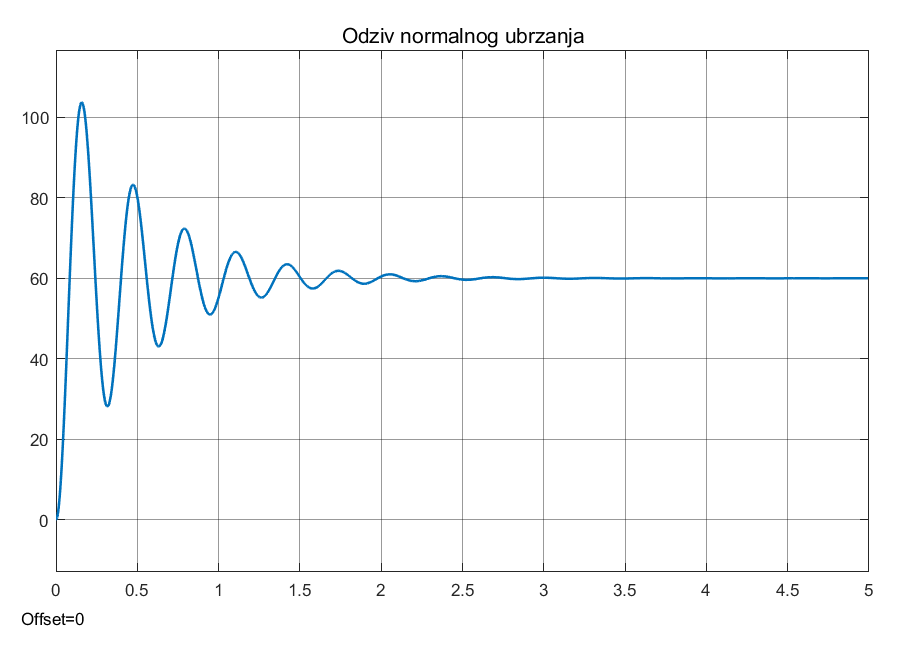
\includegraphics[scale = 0.6]{nZodziv.eps}
    \caption{Odziv normalnog ubrzanja na odskočni otklon krmila visine}
    \label{fig:nLodziv}
\end{figure}
Ako se uvede povratna sprega po normalnom ubrzanju pomoću akcelerometra kao na slici \ref{fig:akcLoop},
tada je prenosna funkcija zatvorene petlje:
\begin{equation}
    \frac{n_L(s)}{u(s)} = \frac{KV}{T^2s^2+2\xi Ts + 1 +K_{akc}KV}
\end{equation}
\begin{figure}[!ht]
    \centering
    \begin{tikzpicture}[auto, node distance=2cm,>=latex']
        \node[input, name=input](input){};
       \node[sum, right of = input](sum){};
       \node[block, right of = sum] (g1){$\frac{KT_1}{T^2s^2+2\xi Ts+1}$};
       \node[block, right of = g1,node distance = 2.5cm] (g2){$\frac{V}{T1}$};
       \node [output, right of = g2] (output) {};
       \node[block, below of = g1] (gyro){$K_{akc}$};
       \draw [->] (g2) -- node [name=y, anchor = south] {$n_L$}(output);
       \draw[->] (y)|-(gyro);
       \draw[->] (gyro) -|node[pos=0.99] {$-$}(sum);
       \draw[->](g1) -- (g2);
       \draw [draw,->] (input) -- node {$u$} node[pos=0.99] {$+$}(sum);
       \node[anchor = south] (thetadot) at ($(g1)!0.6!(g2)$){$\alpha$};
       \draw[->] (sum)--(g1);
    \end{tikzpicture}
    \caption{Blok dijagram sistem za upravljanje normalnim ubrzanjem}
    \label{fig:akcLoop}
\end{figure}
Korištenjem teoreme o konačnoj vrijednosti dobija se da je stacionarna vrijednost 
na odskočnu pobudu sistema sa zatvorenom spregom sada $\frac{KV}{1+K_{akc}KV}$. 
Za velike vrijednosti pojačanja povratne sprege ima se da je stacionarna vrijednost odziva 
$1/K_{akc}$ pa na prvi pogled izgleda da se može postići proizvoljno pojačanje ali treba 
uzeti u obzir da ubrzanje projektila može lahko doći u zasićenje i da isto tako 
otklon krmila može dostići maksimalnu vrijednost. Sopstvena frekvencija sistema 
sa zatvorenom spregom je sada povećana i iznosi $\frac{1+K_{akc}KV}{T^2}$ a novi 
koeficijent prigušenja je smanjen i iznosi $\xi (1+K_{akc}KV)^{-1/2}$. Ovo nije dobra 
osobina s obzirom da se od autopilota zahtjeva da poveća koeficijent prigušenja kako bi 
se povećala stabilnost sistema. Generalno, performanse projektila su obično 
manje od zahtjevanih pa je uvijek zadatak autopilota da ih poboljša. 
Odziv normalnog ubrzanja sa zatvorenom spregom po ubrzanju je prikazan na slici \ref{fig:akcClosed}.
\begin{figure}[!ht]
    \centering
    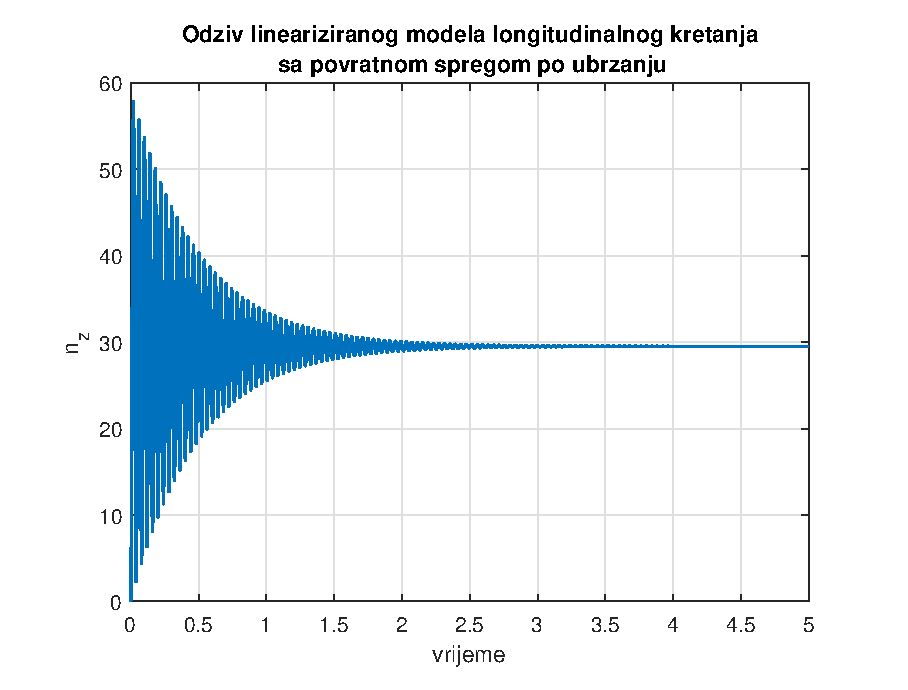
\includegraphics[scale = 0.6]{akcClosed.eps}
    \caption{Odziv normalnog ubrzanja sa zatvorenom spregom po ubrzanju je prikazan}
    \label{fig:akcClosed}
\end{figure}
Jasno se sa grafika vidi da su oscilacije povećane jer je smanjen koeficijent prigušenja. 
Da bi se nadoknadio smanjeni koeficijent prigušenja, u svrhu njegova povećanja može se uvesti 
nova povratna sprega po brzini promjene ugla propinjanja kao što je to prikazano na slici 
\ref{fig:nz2loop}
\begin{figure}[!ht]
    \centering 
    \begin{tikzpicture}[auto, node distance=2cm,>=latex',scale = 1.5]
        \node[input, name=input](input){};
       \node[sum, right of = input](sum){};
       \node[block, right of = sum] (g1){$\frac{K(T_1s+1)}{T^2s^@+2\xi Ts+1}$};
       \node[block, right of = g1,node distance = 3cm] (g2){$\frac{V}{T_1s+1}$};
       \node[output, right of = g2,node distance = 3cm](out){};
       \node[anchor = south] (thetadot) at ($(g1)!0.6!(g2)$){$\dot{\theta}$};
       \node[block,below of = thetadot] (k){$K_{GB}$};
       \node[sum, below of = k,node distance = 1.5cm](sum2){};
       \node[block, right of = sum2](gy){$K_{akc}$};
       \draw[->](g2)--node[name = y, anchor = south]{$n_L$}(out);
       \draw[draw,->] (input) -- node[]{$u$}node[pos=0.99]{$+$}(sum);
       \draw[->](sum)--(g1);
       \draw[->](g1)--(g2);
       \draw[->] (thetadot)--(k);
       \draw[->](k)--node[pos=0.99,anchor = east]{$+$}(sum2);
       \draw[->] (y) |- (gy);
       \draw[->] (gy)--node[pos = 0.99]{$+$}(sum2);
       \draw[->] (sum2) -|node[pos = 0.99]{$-$}(sum);
\end{tikzpicture}
    \caption{Upravljanje normalnim ubrzanjem sa akcelerometrom i brzinskim žiroskopom}
    \label{fig:nz2loop}
\end{figure}
Sada je prenosna funkcija zatvorene petlje data sa:
\begin{equation}
    \frac{n_L(s)}{u(s)} = \frac{KV}{T^2s^2 + (2\xi T+KK_{GB}T_1)s + 1+KK_{GB}+KK_{akc}V}
\end{equation}
Sada je nova stacionaran vrijednost odziva:
\begin{equation*}
    n_{L_{stac}} = \frac{KV}{ 1+KK_{GB}+KK_{akc}V}
    \label{eq:stac}
\end{equation*}
,a novi faktor prigušenja je dat sa:
\begin{equation*}
    \xi ' = \frac{1}{2}\frac{2\xi T+KK_GT_1}{\sqrt{1+KK_G+KK_{akc}V}}
\end{equation*}
I nova prirodna frekvencija je određena sa:
\begin{equation*}
    \omega _n' =\frac{\sqrt{1+KK_G+KK_{akc}V}}{T} 
\end{equation*}
Odziv za referentnu vrijednost $60 \frac{m}{s^2}$ je dat na slici \ref{fig:acc2loopsres}
\begin{figure}[!ht]
    \centering
    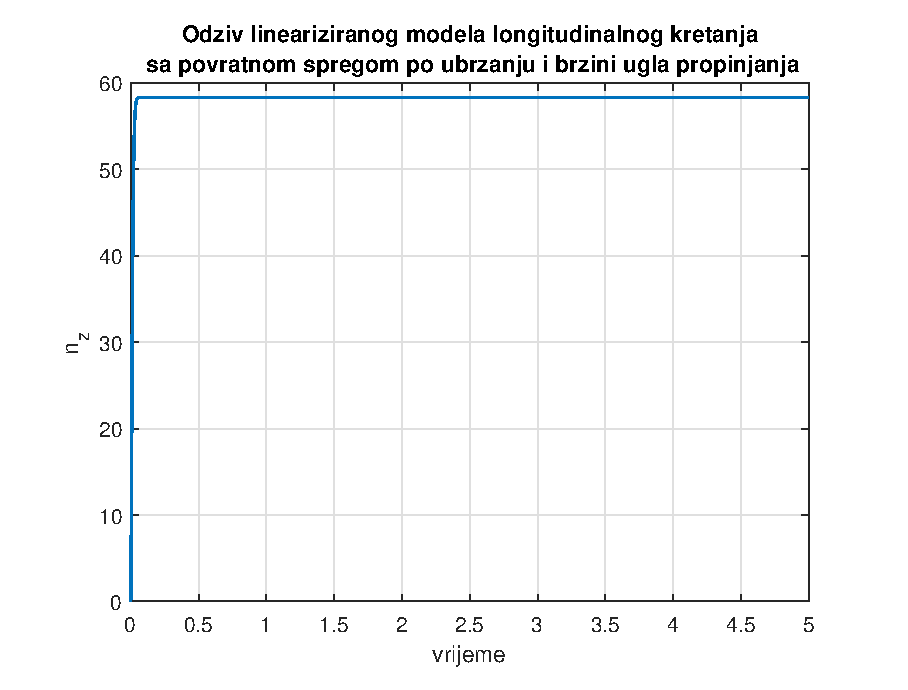
\includegraphics{twoLoopsAcc.eps}
    \caption{Odziv sistema sa povratnom spregom po ubrzanju i brzini ugla propinjanja}
    \label{fig:acc2loopsres}
\end{figure}
Vidi se sa grafika na slici \ref{fig:acc2loopsres} da odziv ne prati referentnu vrijednost. 
Naravno, iz jednačine \ref{eq:stac} se vidi da ako se uzme pojačanje akcelerometra $K_{akc} =1- \frac{1+KK_{GB}}{KV}$
da će se eliminisati greška stacionarnog stanja, ali ovo je naivno rješenje pošto sada pojačanje 
akcelerometra zavisi od parametara projektila koji se mjenjaju sa uslovima leta. Robusnije rješenje je 
uvesti PI regulator u direktnu granu(sl. \ref{fig:pir}) kako bi se eliminisala greška stacionarnog stanja. 
\begin{figure}[!ht]
    \centering
    \begin{tikzpicture}[auto, node distance=2cm,>=latex']
        \node[input, name=input](input){};
       \node[sum, right of = input](sum){};
       \node[sum, right of = sum](sum2){};
       \node[block, right of = sum2](pi){$K_i\frac{1+T_is}{s}$};
       \node[block, right of = pi, node distance = 3cm] (g1){$\frac{K(T_1s+1)}{T^2s^2+2\xi Ts+1}$};
       \node[block, right of = g1,node distance = 2.5cm] (g2){$\frac{V}{1+T_1s}$};
       \node [output, right of = g2] (output) {};
       \node[] (mid) at ($(pi)!0.45!(g1)$){};
       \node[block, below of = mid,node distance = 1.5cm] (g){$K_{GB}$};
       \node[block, below of = g,node distance = 1.5cm] (gyro){$K_{akc}$};
       \draw [->] (g2) -- node [name=y, anchor = south] {$n_L$}(output);
       \draw[->] (y)|-(gyro);
       \draw[->] (gyro) -|node[pos=0.99] {$-$}(sum);
       \draw[->](g1) -- (g2);
       \draw [draw,->] (input) -- node {$u$} node[pos=0.99] {$+$}(sum);
       \draw[->](sum)--node[pos = 0.99]{$+$}(sum2);
       \node[anchor = south] (thetadot) at ($(g1)!0.6!(g2)$){$\dot{\theta}$};
       \draw[->] (sum2)--(pi);
       \draw[->](pi)--(g1);
       \draw[->](thetadot)|-(g);
       \draw[->](g)-|node[pos =0.99]{$-$}(sum2);
\end{tikzpicture}
\caption{PI regulacija normalnog ubrzanja}
\label{fig:pir}
\end{figure}
Neka je PI regulator dat prenosnom funkcijom:
\begin{equation}
    G_{PI} = K_i\frac{1+T_is}{s}
\end{equation}
Ako se tačka u kojoj je $\dot{\theta}$ izmjesti nakon bloka $\frac{V}{1+T_1s}$ dobijaju se 
dvije povratne petlje po istoj veličini pa se mogu pretvoriti u jednu povratnu petlju. Tada je 
pojačanje povratne petlje dato sa:
\begin{equation}
    L(s) = K_{akc}+K_{GB}\frac{1+T_1s}{s}
\end{equation}
a pojačanje direktne grane je:
\begin{equation}
    P(s)=K_i\frac{1+T_is}{s}\frac{KV}{T^2s^2+2\xi Ts+1}
\end{equation}
Sada se nakon dosta algebre dolazi do ukupne prenosne funkcije:
\begin{equation}
    M(s)=\frac{K_iKV(1+T_is)}{T^2s^3+a_2s^2+a_1s + a_0}
\end{equation}
gdje je:
\begin{align*}
    & a_2 = 2\xi T+K_{GB}K_iKT_iT_1 \\
    & a_1 = 1+K_iK_{akc}KVT_i+K_{GB}K_iK(T_i+T_1)\\
    & a_0 = K_{akc}KVK_i+K_{GB}K_iK
\end{align*}
Sada je stacionarna vrijednost odziva na odskočnu pobudu:
\begin{equation}
    n_{L_{stac}} = \frac{K_iKV}{K_{akc}KVK_i+K_{GB}K_iK} = \frac{V}{K_{akc}V+K_{GB}}
\end{equation}
Sada, ako se zahtjeva da odziv nema greške stacionarnog stanja, treba odabrati:
\begin{equation}
    K_{akc} = 1-\frac{K_{GB}}{V}
\end{equation}
Ovo je dosta bolje rješenje, budući da ovdje treba poznavati samo brzinu projektila. Parametri 
PI regulatora i pojačanje brzinskog žiroskopa se mogu odabrati da zadovolje neki kriterij. 
Na grafiku \ref{fig:piAcc} je prikazan odziv i vidi se da nema greške stacionarnog stanja. 
Uzeto je jedinično pojačanje brzinskog žiroskopa i prenosna funkcija PI regulatora $G_{PI}=5\frac{1+s}{s}$. 
Ovo je naizgled izvrsno rješenje ali treba uvijek uzeti u obzir da normalno ubrzanje projektila 
može doći u zasićenje i da prevelika ubrzanja mogu dovesti sistem u nestabilno stanje. Također 
maksimalno normalno ubrzanje ograničeno je maksimalnim otklonom krmila visine pa treba koristiti 
anti-windup schemu za upravljanje kako se ne bi akumulirala prevelika greška.  
\begin{figure}[!ht]
    \centering
    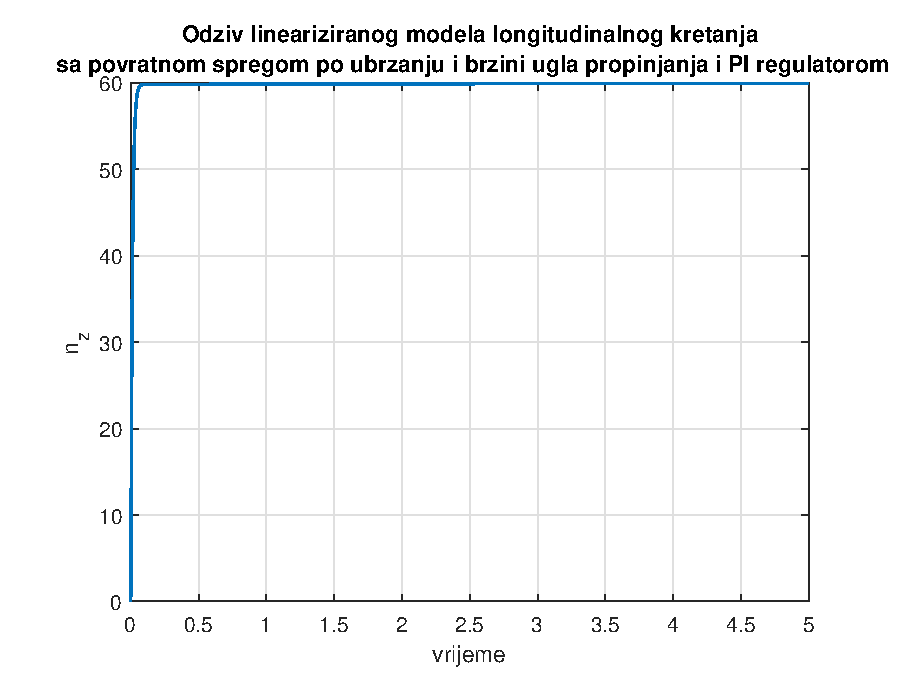
\includegraphics{piAcc.eps}
    \caption{Odziv normalnog ubrzanja sa PI regulatorom i povratnom spregom 
    sa brzinskim žiroskopom i akcelerometrom}
    \label{fig:piAcc}
\end{figure}
Regulacija vertikalnog ubrzanja se može izvršiti i korištenjem feedforward pojačanja. U blok 
dijagramu na slici \ref{fig:ffa}. Ovdje je pojačanje akceleromatra prebačeno nakon sumatora, 
ispred sumatora na ulaz je prebačeno $1/K_{akc}$, pa ako se uzme pojačanje referentnog signala 
od $K_{akc}$ dobije se dijagram na slici. Ovime se osigurava praćenje referentne vrijednosti. Kao i ranije 
faktor prigušenja se podešava pojačanjem brzinkskog žiroskopa.  
\begin{figure}[!ht]
    \centering
    \begin{tikzpicture}[scale = 1,auto, node distance=2cm,>=latex']
    \node[input, name = input](input){};
    \node[sum,right of = input](sum1){};
    \node[block,right of = sum1](pi){$K_{akc}K_i\frac{1+T_is}{s}$};
    \node[sum,right of = pi,node distance = 2.5cm](sum2){};
    \node[block,right of = sum2](model){Model};
    \node[output,right of = model,yshift = 5](psi){};
    \node[output,right of = model,yshift = -5](nh){};
    \node[anchor = east,yshift = 5] at(model.east)(psi1){};
    \node[anchor = east,yshift = -5] at(model.east)(nh1){};
    \node[block,below of =model,xshift = 1](kg){$K_{GB}$};
    \draw[->](input) --node{$a_{V_{ref}}$+}(sum1);
    \draw[->](sum1)--(pi);
    \draw[->](pi)-- node[pos = 0.99]{$+$}(sum2);
    \draw[->](sum2)--(model);
    \draw[->](psi1)-- node[name = psiout,anchor = south east]{$\dot{\theta}$}(psi);
    \draw[->](nh1)-- node[name = nhout,anchor = south]{$a_{V}$}(nh);
    \draw[->](psiout)|-(kg);
    \draw[->](kg)-|node[pos = 0.99]{$-$}(sum2);
    \draw[->](nhout) |- ++(0,-3) -| node[pos = 0.99]{$-$}(sum1);
    \end{tikzpicture}
    \caption{Regulator za upravljanje vertikalnim ubrzanjem}
    \label{fig:ffa}
    \end{figure}
\section{Regulator za horizontalno ubrzanje}
Kod projektila krstaste konfiguracije dinamika u kanalu pravca je ista kao i dinamika u kanalu visine. 
Ovakav zaključak se može opravdati posmatrajući diferencijalne jednačine koje opisuju 
rotaciju u kanalu visine(propinjanja) i kanalu pravca(zakretanja). 
\begin{align*}
    \frac{dQ}{dt} &= PR\frac{I_z-I_x}{I_y} + M/I_y\\
    \frac{dR}{dt} &= PQ\frac{I_x-I_y}{I_y} + N/I_z
\end{align*}
Sjetimo se da su koeficjenti kod momenta zakretanja i momenta skretanja isti, ali različitog znaka i da vrijedi $I_z = I_y $. 
To znači da će regulator horiznotalnog ubrzanja biti isti kao i regulator 
vertikalnog ubrzanja uz jednu bitnu razliku. U poglavlju o modelu, pokazano je da je odziv ugla zakretanja 
za pozitivan otklon krmila pravca negativan, za razliku odziva ugla propinjanja na pozitvan otklon krmila pravca koji je 
pozitivan. Ovo znači da se za korektnu regulaciju horizontalnog ubrzanja treba promjeniti znak 
otklona krmila pravca. 
\begin{figure}[!ht]
    \centering
    \begin{tikzpicture}[scale = 0.15,auto, node distance=2cm,>=latex']
    \node[input, name = input](input){};
    \node[sum,right of = input](sum1){};
    \node[block,right of = sum1](pi){$K_{akc}K_i\frac{1+T_is}{s}$};
    \node[sum,right of = pi,node distance = 2.5cm](sum2){};
    \node[block,right of = sum2](minus){$-1$};
    \node[block,right of = minus](model){Model};
    \node[output,right of = model,yshift = 5](psi){};
    \node[output,right of = model,yshift = -5](nh){};
    \node[anchor = east,yshift = 5] at(model.east)(psi1){};
    \node[anchor = east,yshift = -5] at(model.east)(nh1){};
    \node[block,below of =minus,xshift = 1](kg){$K_{GB}$};
    \node[below of = pi,node distance = 4cm](mid){};
    \draw[->] (input) --node{$a_{H_{ref}}$+}(sum1);
    \draw[->](sum1)--(pi);
    \draw[->](pi)-- node[pos = 0.99]{$+$}(sum2);
    \draw[->](sum2) -- (minus);
    \draw[->](minus)--(model);
    \draw[->](psi1)-- node[name = psiout,anchor = south east]{$\dot{\psi}$}(psi);
    \draw[->](nh1)-- node[name = nhout,anchor = south]{$a_{H}$}(nh);
    \draw[->](psiout)|-(kg);
    \draw[->](kg)-|node[pos = 0.99]{$-$}(sum2);
    \draw[->](nhout) |- ++(0,-20) -| node[pos = 0.99]{$-$}(sum1);
    \end{tikzpicture}
    \caption{Regulator za upravljanje horizontalnim ubrzanjem}
    \end{figure}
\section{Stabilizacija ugla valjanja}
Sada je trenutak da se spomenu dvije vrste letjelica. Neke letjelice koje imaju izražene 
krilne površine(npr. komercijalni i borbeni avioni) vrše rotaciju oko longitudinalne ose kako 
bi izvršile manevre u horizontalnoj ravnini. Letjelice koje operiraju na ovakav način se 
generalno zovu "bank-to-turn" ili "valjati-za-skretanje". Ovo znači da ako letjelica 
treba da promjeni ugao zakretanja mora izvršiti valjanje oko longitudinalne ose kako bi se 
generisala sila uzgona koja bi za posljedicu imala kretanje u vertikalnoj ravni. Neki stariji 
protiv-tenkovski projektili koji imaju samo jedan par kontrolnih površina koriste ovakvu konfiguraciju, ali 
su oni danas zamjenjeni boljim projektilima. Kada se radi o projektilima koji imaju dva para kontrolnih površina 
moguće je izazvati kretanje u vertikalnoj i horizontalnoj ravni bez potrebe za valjanjem. Sjetimo se da 
pojava valjanja izaziva unakrsnu spregu kanala zakretanja i kanala visine pa je ovakav tip upravljanja projektila dosta 
bolji ako projektil posjeduje dva para krila. Ovakva konfiguracija letjelica se zove "skid-to-turn" ili "klizati-za-skretanje". 
Prema tome, kod projektila krstaste konfiguracije za realizaciju "skid-to-turn" manevara mora se stabilizirati kanal valjanja. 
Za stabilizaciju i za upravljnje kanalom valjanja koristi se isti regulator, koji je sličan regulatorima za vertikalno i 
horiznotalno ubrzanje. Struktura regulatora za stabilizaciju ugla valjanja je prikazana na slici \ref{fig:rollStab}.
\begin{figure}[!ht]
    \centering
    \begin{tikzpicture}[auto, node distance=2cm,>=latex']
        \node[input,name=input](input){};
        \node[sum,right of = input](sum1){};
        \node[block, right of = sum1,node distance = 2cm](pi1){$PI$};
        \node[sum, right of = pi1,node distance = 2.5cm](sum2){};
        \node[block, right of = sum2](pi2){$PI$};
        \node[block, right of = pi2](model){Model};
        \node[anchor = east,yshift = 10] at (model.east)(p){};
        \node[output, right of=model, yshift = 10](pout){};
        \node[] (priv) at ($(pi2)!0.5!(model)$){};
        \node[block,below of = priv](kg){$K_{GB}$};
        \node[anchor = east,yshift = -10] at (model.east)(phi){};
        \node[output,right of = model, yshift=-10](phiout){};
        \draw[->](phi)--node[name=phiout1, anchor = south west]{$\phi$}(phiout);
        \draw[->](phiout1) |- ++(0,-3) -| node[pos=0.99]{$-$}(sum1);
        \draw[->](kg) -| node[pos=0.99]{$-$}(sum2);
        \draw[->](p)--node[name=pout1]{$P$}(pout);
        \draw[->](pi2)--(model);
        \draw[->](sum2)--(pi2);
        \draw[->](pi1)--node[pos=0.99]{$+$}(sum2);
        \draw[->](sum1)--(pi1);
        \draw[->](input)--node[pos = 0.5]{$\phi = 0$+}(sum1);
        \draw[->](pout1) |- (kg);
        \end{tikzpicture}
    \caption{Regulator za stabilizaciju ugla valjana}
    \label{fig:rollStab}
\end{figure}
\section{Autopilot za skid-to-turn projektil}
U nastavku je prikazan nelinearni model projektila krstate konfiguracije sa tri 
prethodno predstavljena regulatora. Ovaj autopilot je samo jedan korak daleko od
implemenatcije kompletnog sistema vođenja projektila kratkog dometa proporcionalnom
navigacijom. Na slci \ref{fig:autopilot3}
\begin{figure}[!ht]
    \centering
    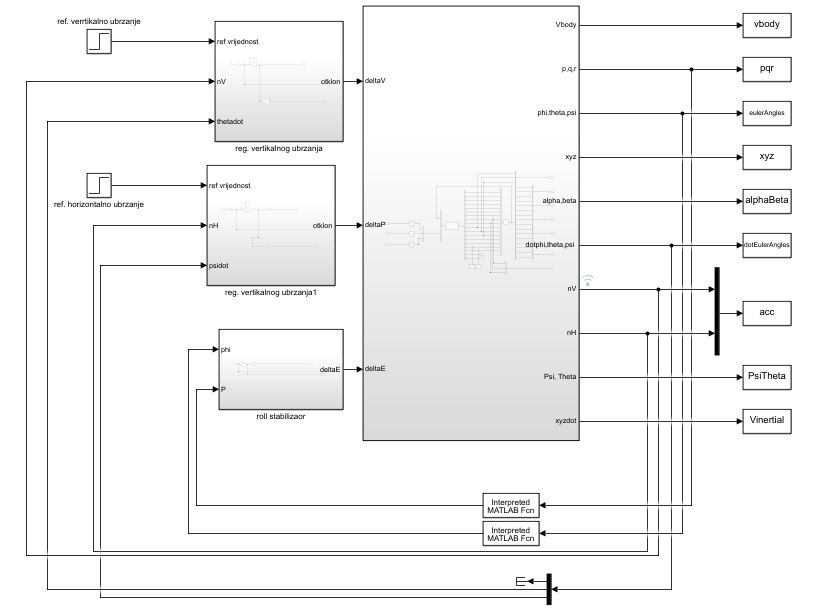
\includegraphics[scale = 0.6]{autopilot.JPG}
    \caption{Model sa autopilotom}
    \label{fig:autopilot3}
\end{figure}
U ovom simulink dijagramu su prethodno predstavljeni regulatori za vertikalno i normalno ubrzanje i 
regulator za stabilizaciju ugla valjanja sublimirani u simulink podsisteme radi 
urednosti dijagrama. Dvije interpretirane Matlab funkcije služe samo za izdvajanje ugaone brzine valjanja
i ugla valjanja. U nastavku će se na nekoliko primjera ispitati performanse 
autopilota. Prvo je prikazan odziv kada se zahtjeva konstantno vertikalno ubrzanje i nulto 
horizontalno ubrzanje. Ovakav zahtjev je čest u praksi, jer predstavlja vođenje projektila 
prema meti koja se nalazi upravo u ravni $xz$ projektila. Na slici \ref{fig:accautover} su prikazani 
ubrzanja i orijentacija projektila kada se zahtjeva vertikalno ubrzanje od $20 m/s^2$ i horiznotalno ubrzanje od 
$0m/s^2$.
\begin{figure}[!ht]
    \centering
    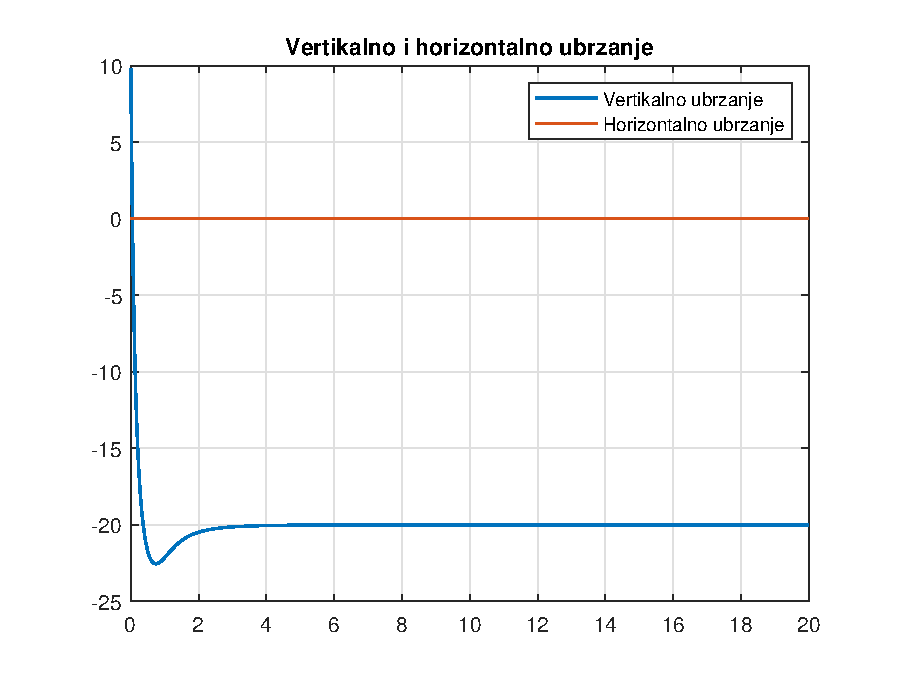
\includegraphics[scale = 0.5]{accautopilotver.eps}
    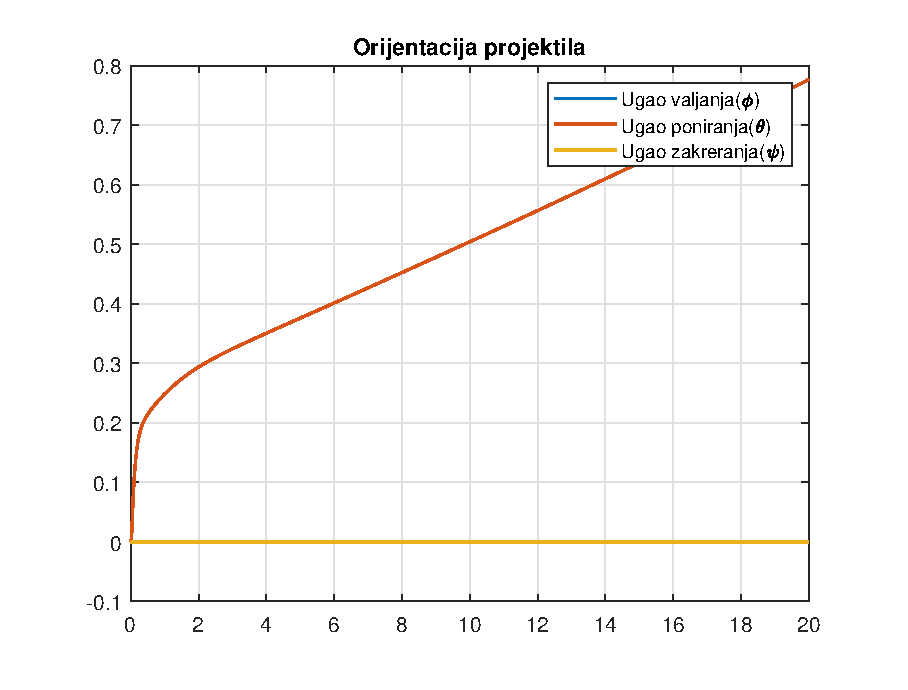
\includegraphics[scale = 0.5]{eulerAutoVer.eps}
    \caption{Ubrzanja i orijentacija projektila sa autopilotom pri longitudinalnom kretanju}
    \label{fig:accautover}
\end{figure}
Vidi se da projektil prati zadata ubrzanja i da je stabilisan kanal valjanja. Ugao propinjanja raste, 
što govori o činjenici da se projektil kreće po dijelu kružnice pa ako bi se izvršila duža simulacija 
uvidjelo bi se da projektil pravi petlje u $xz$ ravnini. Vidi se da je ugao zakretanja 
uvijek nula, što govori da projektil ne čini pomjeraje u vertikalnoj ravnini. U ovom primjeru se 
vidi da je autopilot zadovoljio zahtjevane performanse. Važno je istaći se kod upravljanja vertikalnim 
ubrzanjem, kod ovog modela, javlja zasićenje za $25m/s^2$. Ovo je najveći problem 
kod vođenja projektila jer upravo ovaj problem izaziva promašaj. 
Pogledajmo sada odziv sistema kada se zahtjeva nulto vertikalno i horizontalno ubrzanje od $20m/s^2$. 
Ubrzanja i orijentacija su prikazani na slici \ref{fig:horOdziv}.
\begin{figure}[!ht]
    \centering
    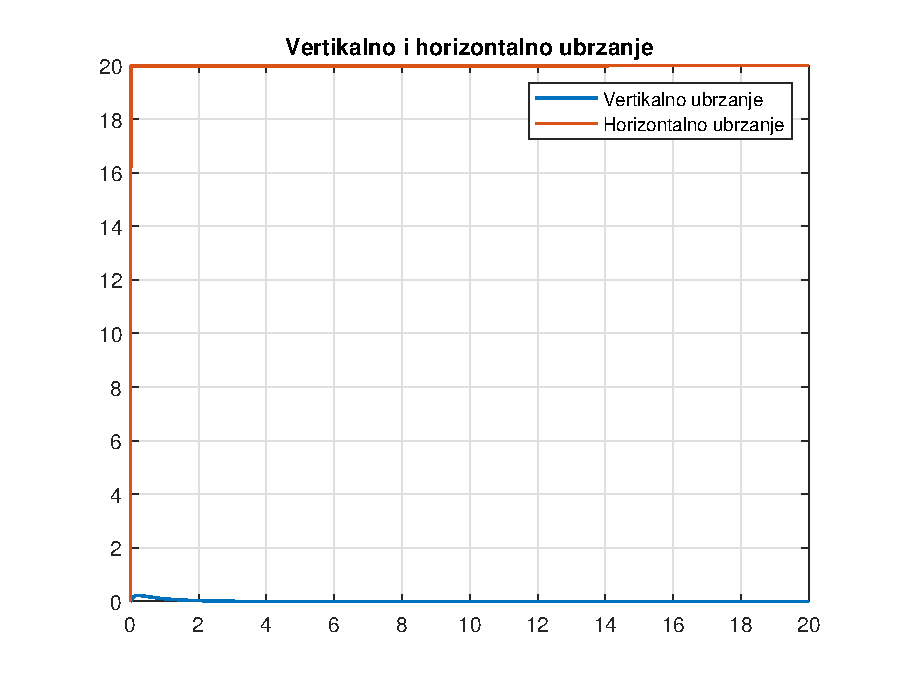
\includegraphics[scale = 0.5]{accHor.eps}
    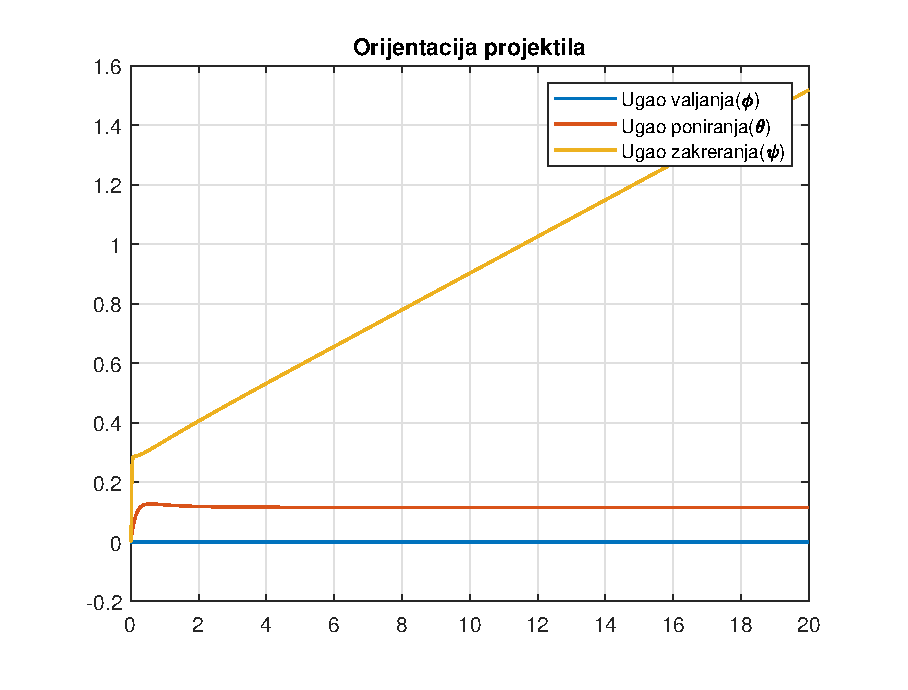
\includegraphics[scale = 0.5]{eulerHor.eps}
    \caption{Ubrzanja i orijentacija projektila sa autopilotom pri lateralnom kretanju}
    \label{fig:horOdziv}
\end{figure}
Opet se vidi da autopilot zadovaljava zadate reference. Vidi se da je odziv horizontalnog 
ubrzanja dosta brži od odziva vertikalnog ubrzanja. Ovo je posljedica nepostojanja 
gravitacione sile u vertikalnoj ravni. Vidi se da je ugao valjanja stalno nula, i da zbog 
kretanja u vertikalnoj ravni ugao zakretanja se mijenja. Ugao propinjanja opada što 
znači da se projektil usmjerava ka zemlji. Ponovo, ovo je posljedica sile uzgona na 
aerodinamički centar pritiska. Odavde slijedi da projektil propada, tj. da se kreće ka dole, ali da pravi 
kružnu putanju u vertikalnoj ravnini. Ovo se vidi na slici \ref{fig:horxyz}.
\begin{figure}[!ht]
    \centering 
    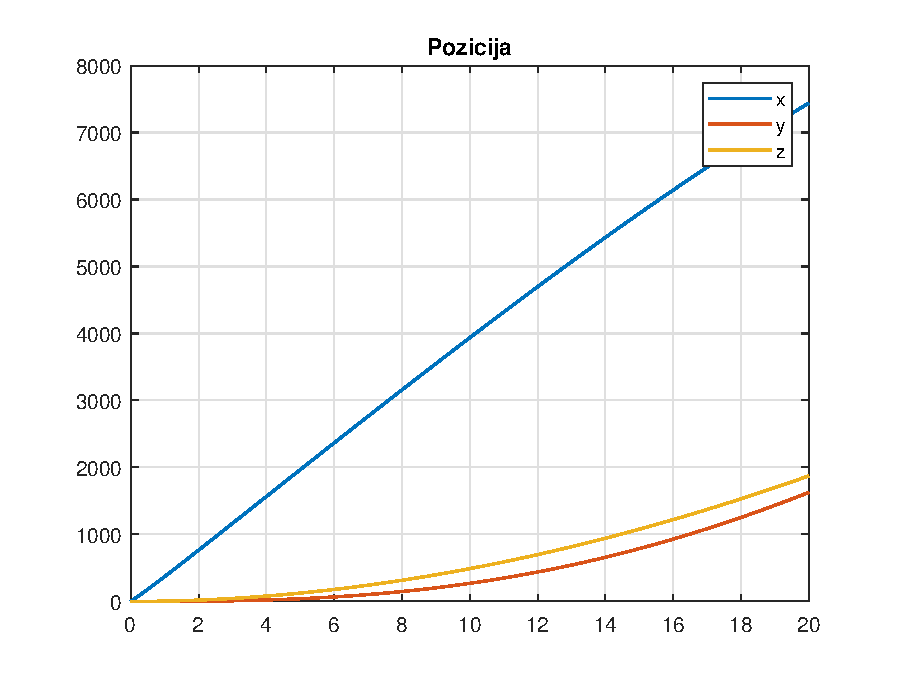
\includegraphics[scale=0.6]{xyzHor.eps}
    \caption{Koordinate projektila u inercijalnom sistemu }
    \label{fig:horxyz}
\end{figure}
Sjetimo se da je $z$ osa inercijalnog sistema usmjerena ka centru Zemlje, pa je sa slike očito da 
je projektil u slobodnom padu u vertikalnoj ravnini. 
Sada posmatrajmo kombinovano kretanje. Neka se zahtjeva i vertikalno i horizontalno 
ubrzanje iznosa $20m/s^2$. Za očekivati je kombinaciju prethodna dva primjera. 
Odzivi ubrzanja i orijatancija pri lateralnom i longitudinalnom kretanju su prikazani na slici \ref{fig:kombinovano}.
\begin{figure}[!ht]
    \centering
    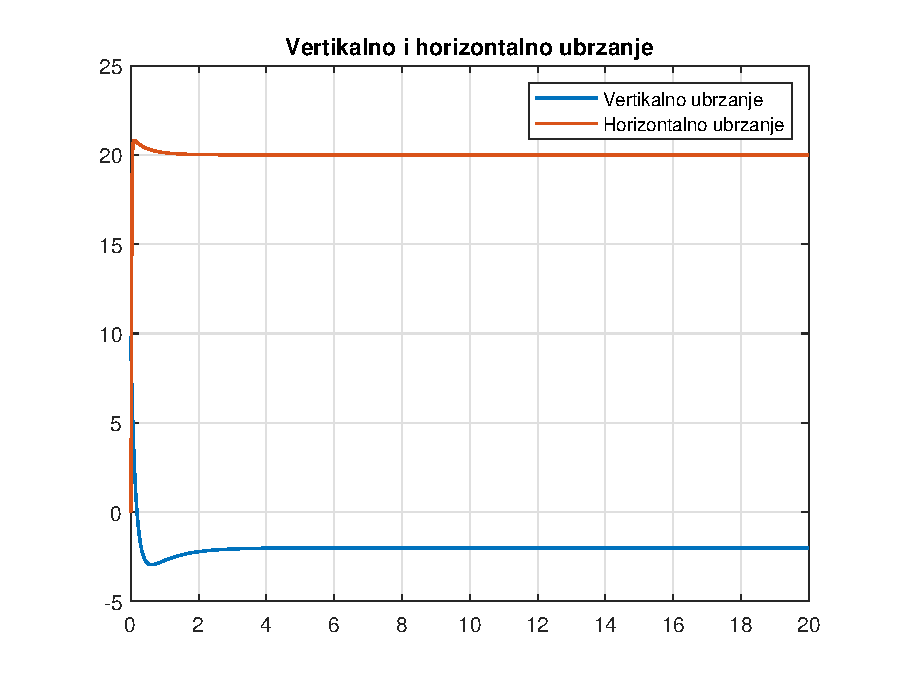
\includegraphics[scale = 0.5]{ubrKomb.eps}
    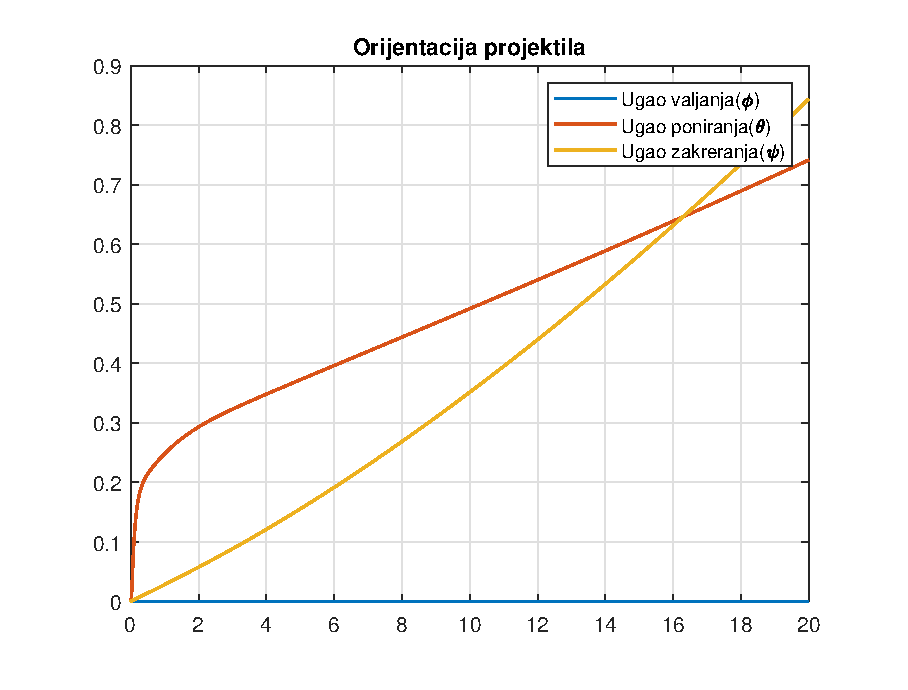
\includegraphics[scale = 0.5]{eulerKomb.eps}
    \caption{Ubrzanja i orijentacija pri lateralnom i longitudinalnom kretanju}
    \label{fig:kombinovano}
\end{figure}
Ovdje se vidi da autopilot i u ovom slučaju zadovoljava zahtjevane performanse. Očekivano i 
ugao poniranja i ugao zakretanja rastu jer se zahtjeva kretanje po dijelu kružnice u obje ravni. 
Ponovo, ugao valjanja je nula tako da se može ostvariti Dekartovo upravljanje, odnosno da 
se ovakav projektil i u najgorem slučaju može voditi proporcionalnom navigacijom.
Regulator za stabiliaziciju valjanja ima jednu zanimljivu osobinu. Iako on osigurava 
da je ugao valjanja nula, on ne osigurava da je ugaona brzina valjanja nula. Drugim riječima, 
projektil se rotira nekom malom ugaonom brzinom oko svoje $x$ ose, ali je njegova orijentacija u kanalu 
valjanja i dalje nula u odnosu na inercijalni sistem. Ugaone brzine tijela projektila oko 
svojih osa su prikazane na slici \ref{fig:angular}.
\begin{figure}[!ht]
    \centering
    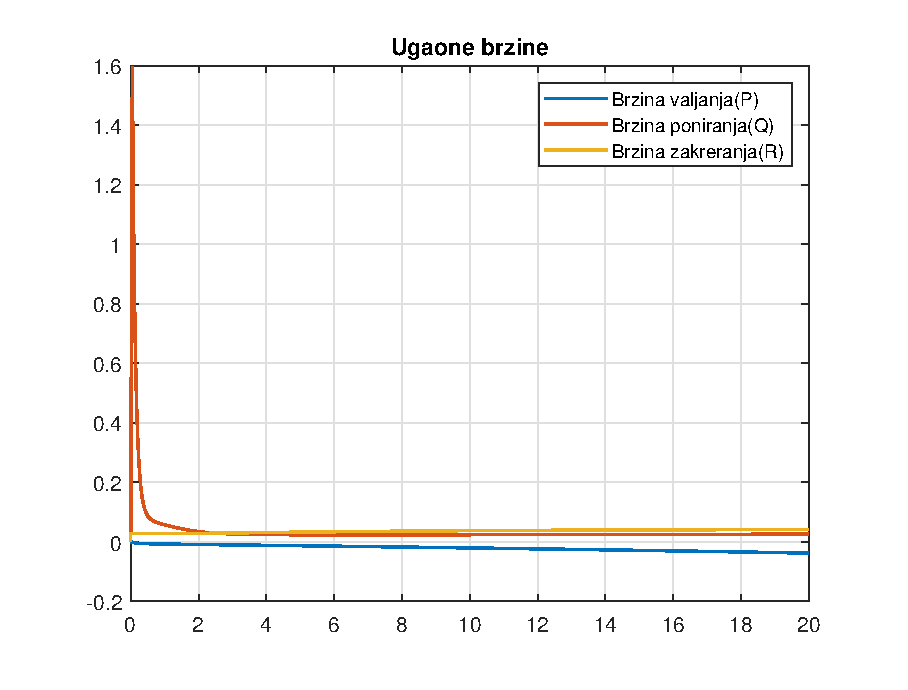
\includegraphics[scale = 0.6]{angular.eps}
    \caption{Ugaone brzine pri lateralnom i longitudinalnom kretanju}
    \label{fig:angular}
\end{figure}
Ovdje se vidi da su ugaone brzine oko sve tri ose sistema tijela različite on nule. 
Za ugaone brzine poniranja i zakretanja ovo je očekivano i neophodno, ali za ugaonu 
brzinu valjanja ovo je iznenađujuće. Ovo slijedi iz činjenice da je promjena ugla valjanja data sa 
$\dot{\phi} =P + Q\sin\phi\tan\theta + R\cos\phi\tan\theta$. Ovo znači da pri postojanju ugaonog kretanja u obje ravni
, da se mora pojaviti i ugaona brzina u kanalu valjanja kako bi brzina promjene ugla valjanja bila nula. 
Jasno je da će ova pojava izazvati spregu kanala visine i kanala pravca, ali to je neophodna 
cijena za stabilizaciju ugla valjanja koji je osnovni preduslov za Dekartovo upravljanje. 

\section{Integracija sistema za vođenje i autopilota}
Sada je predstavljeno sve što je potrebno za vođenje projektila u prostoru.
Ostaje jedino da se izvrši integracija sistema za vođenja i modela sa autopilotom. 
No, prije nego se pođe u integraciju potrebno je skrenuti pažnju na činjenicu da 
proporcionalna navigacija generiše komponente ubrzanja u inercijalnom koordinatnom sistemu, a 
da autopilot upravlja ubrzanjima u koordinatnom sistemu vezanom za vektor brzine. Neophodno 
je izvršiti transformaciju iz sistema vezanog za zemlju u sistem vezan za vektor brzine. 
Transformacija se vrši na sljedeći način:
\begin{align}
 \label{eq:wind1} a_{V} &= a_z\cos\Theta + g\cos\Theta\\ 
 \label{eq:wind2} a_{H} &= a_y\cos\Psi - a_x\sin\Psi
\end{align}
,gdje su $a_x,a_y,a_z$ ubrzanja koja generiše proporcionalna navigacija. 
Sada se ova ubrzanja prosljeđuju autopilotu kao referente vrijednosti. Ako je autopilot 
u stanju da zadovolji ova ubrzanja, tada se garantuje nulti promašaj. 
U nastavku je na slici \ref{fig:fullPN} prikazan simulink dijagram vođenja projektila prema meti čija se brzina i 
početna pozicija može mijenjati. 
\begin{figure}[!ht]
    \centering
    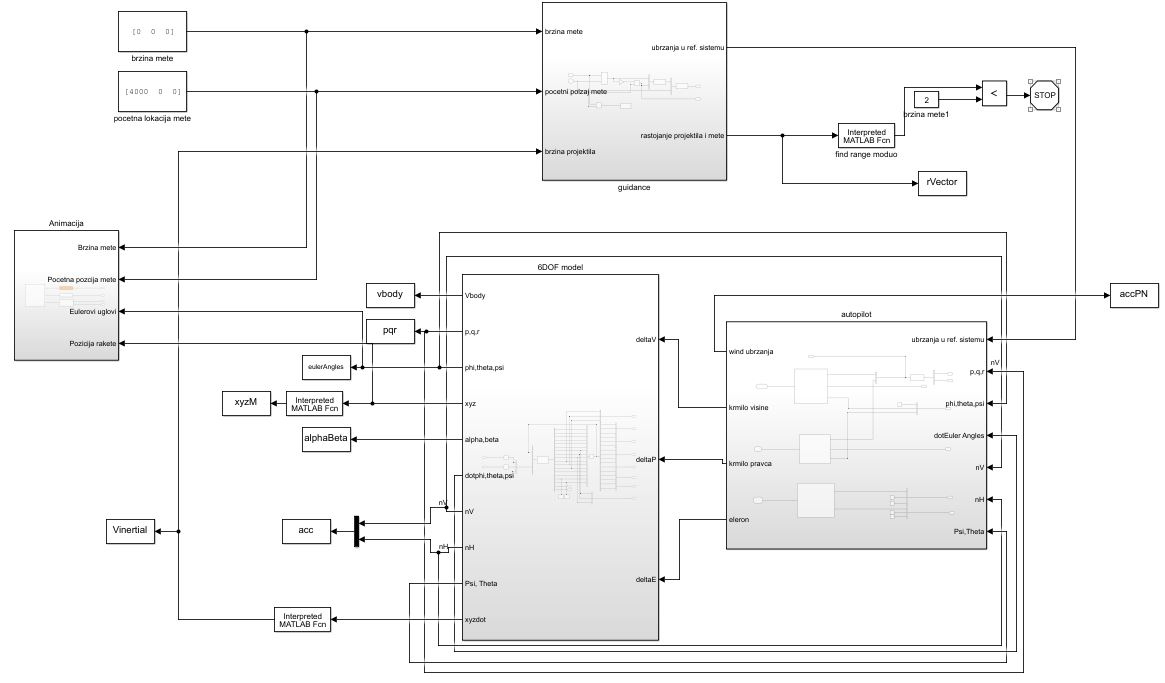
\includegraphics[scale = 0.55]{fullPN.JPG}
    \caption{Simulator za navođenje projektila ka pokretnoj meti}
    \label{fig:fullPN}
\end{figure}
Ovaj simulink dijagram se sastoji iz bloka za proporcionalnu navigaciju koji generiše inerciona ubrzanja, 
zatim iz autopilota koji transformiše ubrzanja iz inercijalnog koordinatnog sistema u 
sistem brzine i koji upravlja ubrzanjima koordinatnog sistema brzine, zatim iz modela sa 
šest stepeni slobode i na kraju iz bloka za animaciju. Ranije je na slici \ref{fig:3dPropFull} u poglavlju 
za proporcionalnu navigaciju predstavljen simulink dijagram koji generiše ubrzanja 
prema zakonu proporcionalne navigacije i radi urednosti neće opet biti predstavljen. 
Važno je samo istaći da simulacija zaustavlja kada udaljenost mete od projektila 
postane dva metra. Ovo je učinjeno radi lakše analize generisanih ubrzanja. Još jedna bitna 
činjenica je da kod proporcionalne navigacije $z$ uzima u smjeru suprotno od 
centra Zemlje, ali se kod modela $z$ osa inercijalnog sistema uzima ka centru Zemlje 
pa je neophodno promjeniti znak brzine u $z$ smjeru pri izlazu iz modela kada se prosljeđuje 
u blok za proporcionalnu navigaciju. 
Podsistem za autopilot je dat na slici \ref{fig:autopilotFull}. 
\begin{figure}[!ht]
    \centering
    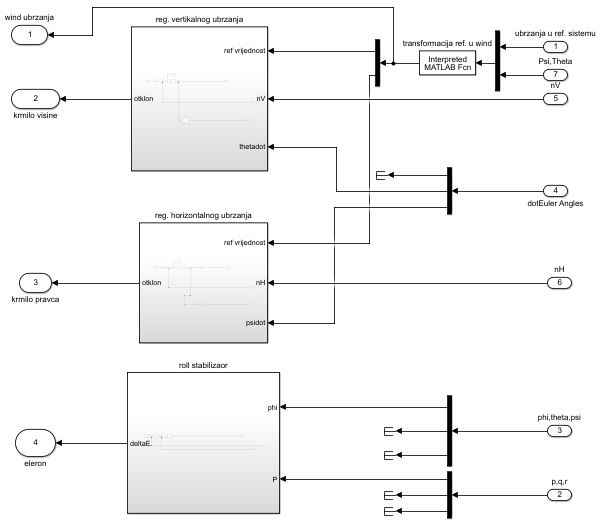
\includegraphics[scale=0.7]{autopilotFull.JPG}
    \caption{Autopilot}
    \label{fig:autopilotFull}
\end{figure}
Ovdje je korištena interpretirana Matlab funkcija koja poziva 
funkciju transform koja je data u nastavku. Ova funkcija transformiše 
ubrzanja data u inercionom sistemu u ubrzanja data u koordinatnom sistemu brzine 
prema relacijama \ref{eq:wind1} i \ref{eq:wind2}.
\begin{lstlisting}
    function out = transform(n,u)
    Psi = u(1);
    Theta = u(2);
    
    nx = n(1);
    ny = n(2);
    nz = n(3);
    
    apitch = nz*cos(Theta) + 9.81*cos(Theta);
    ayaw = ny*cos(Psi) - nx*sin(Psi);
    
    out = [apitch;ayaw];
    end
\end{lstlisting}
Ostali podsistemi su već ranije prikazani regulatori za vertikalno i horizontalno ubrzanje 
i regulator ugla valjanja. 
U svrhu animacije, kreiran je blok za animaciju. Struktura podsistema za animaciju je data na 
slici \ref{fig:animacija}.
\begin{figure}
    \centering
    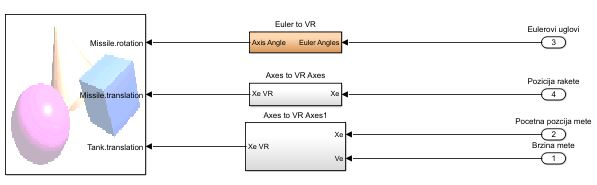
\includegraphics[scale=0.7]{animacija.JPG}
    \caption{Podsistem za animaciju}
    \label{fig:animacija}
\end{figure}
Ovdje je korišten VR sink iz simulink toolbox-a "Virtual reality modeling". 
VR sink interno zahtjeva poziciju projektila i mete i orijentaciju projektila dok se 
meta posmatra kao materijalna tačka, odnosno meta ima samo tri stepena slobode pa ne treba 
prosljeđivati Eulerove uglove. VR sink interno radi sa kvaternionima pa je neophodna konverzija 
iz Eulerovih uglova u kvaretnione.VR sink nam pruža uvid u orijentaciju i 
putanju projektila. Primjer animacije je dat na slici \ref{fig:prAnimacija}.
\begin{figure}
    \centering
    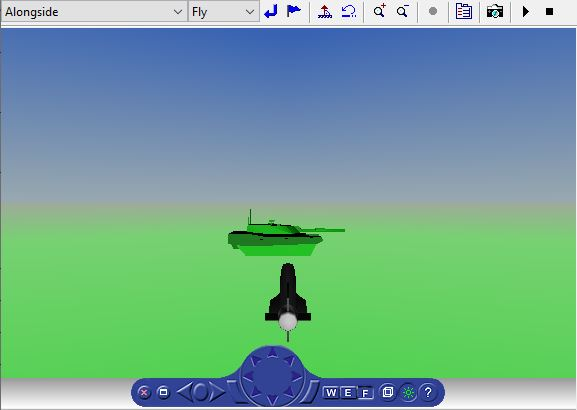
\includegraphics[scale =0.7]{animacijaPr.JPG}
    \caption{Virtual reality modeling}
    \label{fig:prAnimacija}
\end{figure}
U nastavku je prikazan primjer navođenja projektila ka meti koja se nalazi na udaljenosti 
od $4000$ metara i na visini od $100$ metara. 
\begin{figure}[!ht]
    \centering
    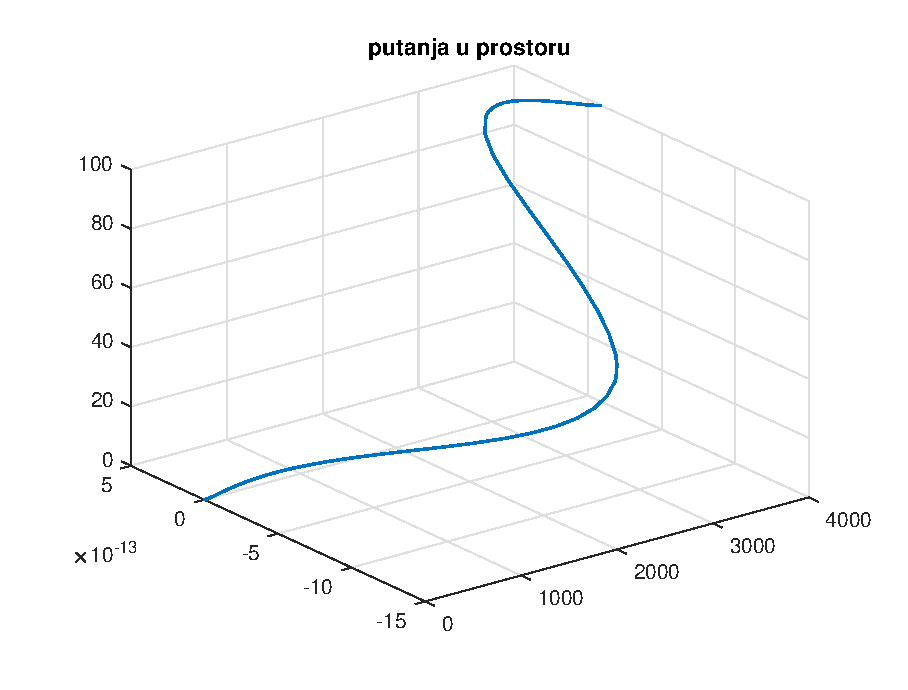
\includegraphics[scale = 0.5]{mtr1.eps}
    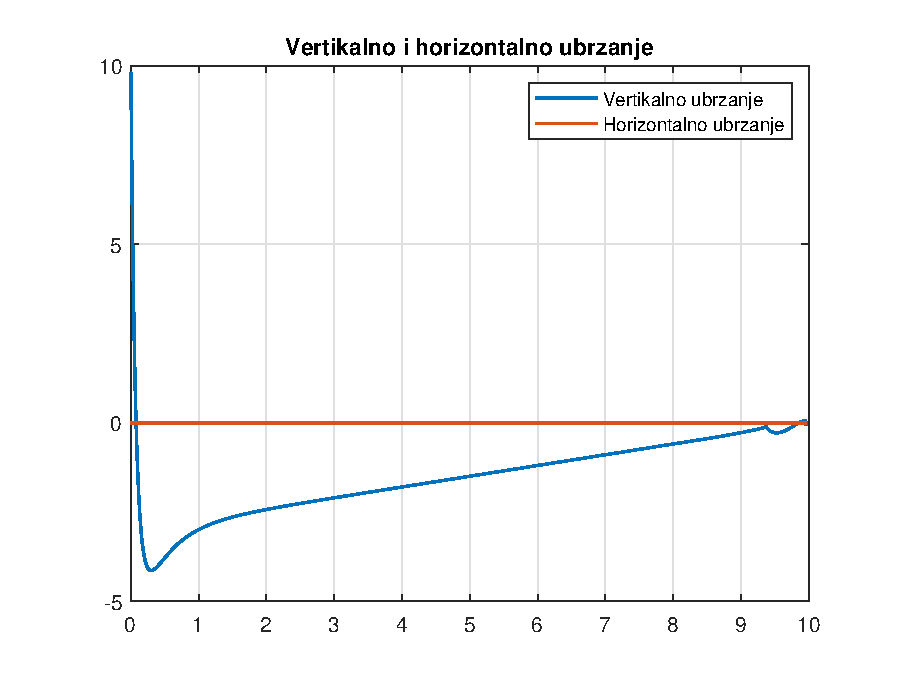
\includegraphics[scale = 0.5]{ub1.eps}
    \caption{Putanja i ubrzanja projektila pri navođenju}
    \label{fig:ub1}
\end{figure}
Na slici \ref{fig:ub1} su prikazani putanja i ubrzanja projektila za ovaj primjer. Vidi se 
da se projektil popeo na visinu od 100 metara i da je presao put od 4000 metara, odnosno da je 
dostigao metu. Gledajući ubrzanja, zahtjeva se da je vertikalno ubrzanje $10m/s^2$, što je 
očekivano jer projektil treba da se penje. Dalje, na slici \ref{fig:or1} se vidi da 
je orijentacije pozitivna čime se postiže sila uzgona koja diže projektil ka meti. 
\begin{figure}[!ht]
    \centering
    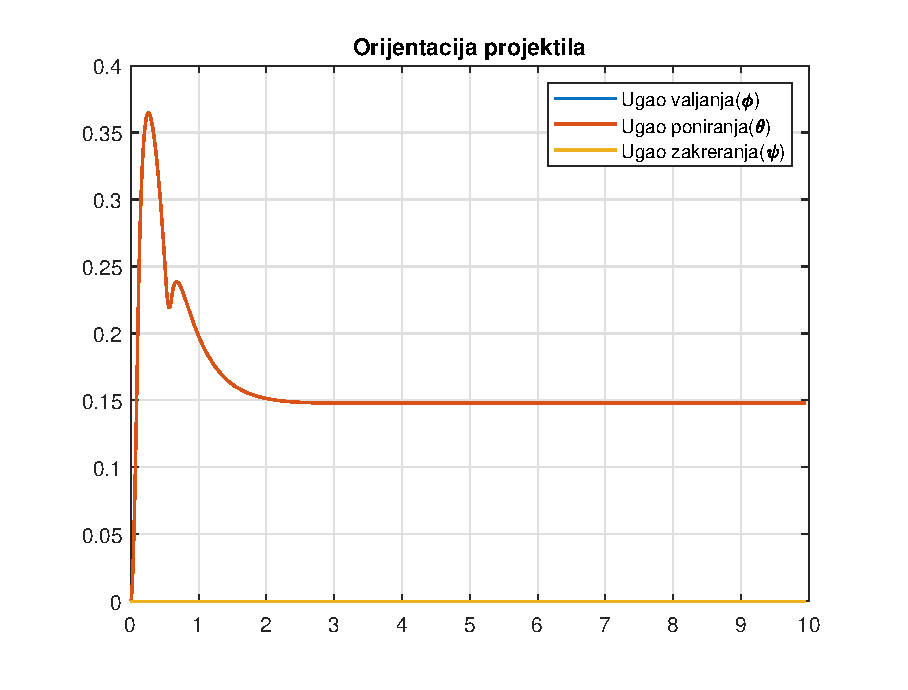
\includegraphics[scale = 0.5]{or1.eps}
    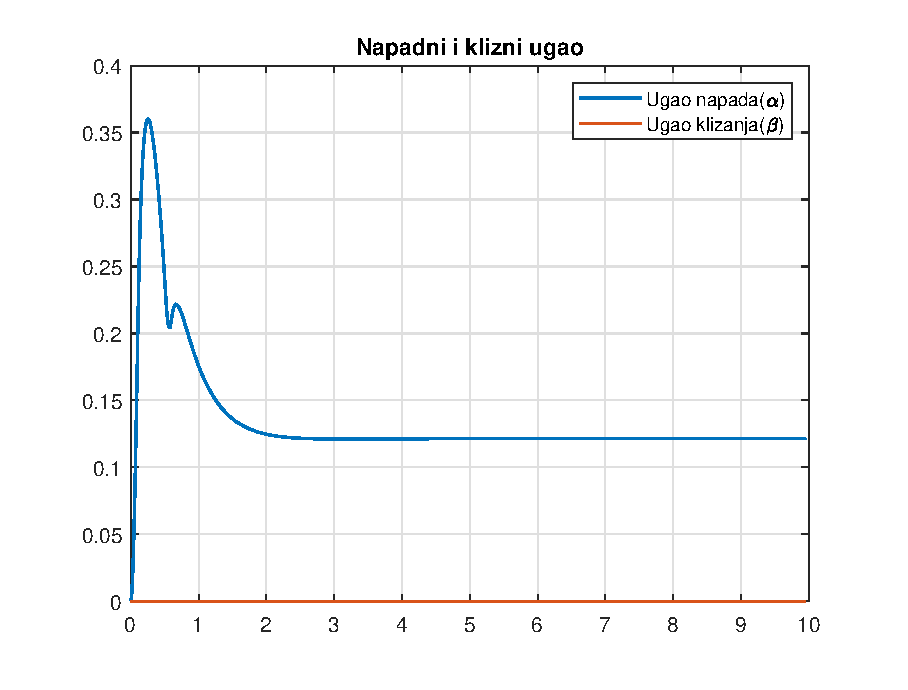
\includegraphics[scale = 0.5]{aoa1.eps}
    \caption{Orijentacija i ugao napada i klizanja projektila pri navođenju}
    \label{fig:or1}
\end{figure}
Vidi se da se održava konstantan pozitivan ugao propinjanja kako bi se osigurala 
sila uzgona da bi se projektil podigao na traženu visinu. Na slici \ref{fig:side1} se 
vidi da je projektil orijentisan ka gore. 
\begin{figure}[!ht]
    \centering
    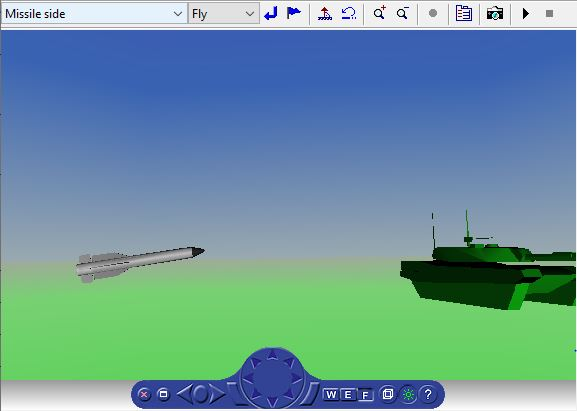
\includegraphics[scale=0.7]{side1.JPG}
    \caption{Projektil neposredno prije susreta}
    \label{fig:side1}
\end{figure}
Sada posmatramo primjer navođenja projektila gdje se meta kreće brzinom $[-10\quad 10\quad 10\quad]^T m/s$.
Na slici \ref{fig:ganja2} je prikazana putanja mete i projektila za ovaj slučaj. 
\begin{figure}[!ht]
    \centering
    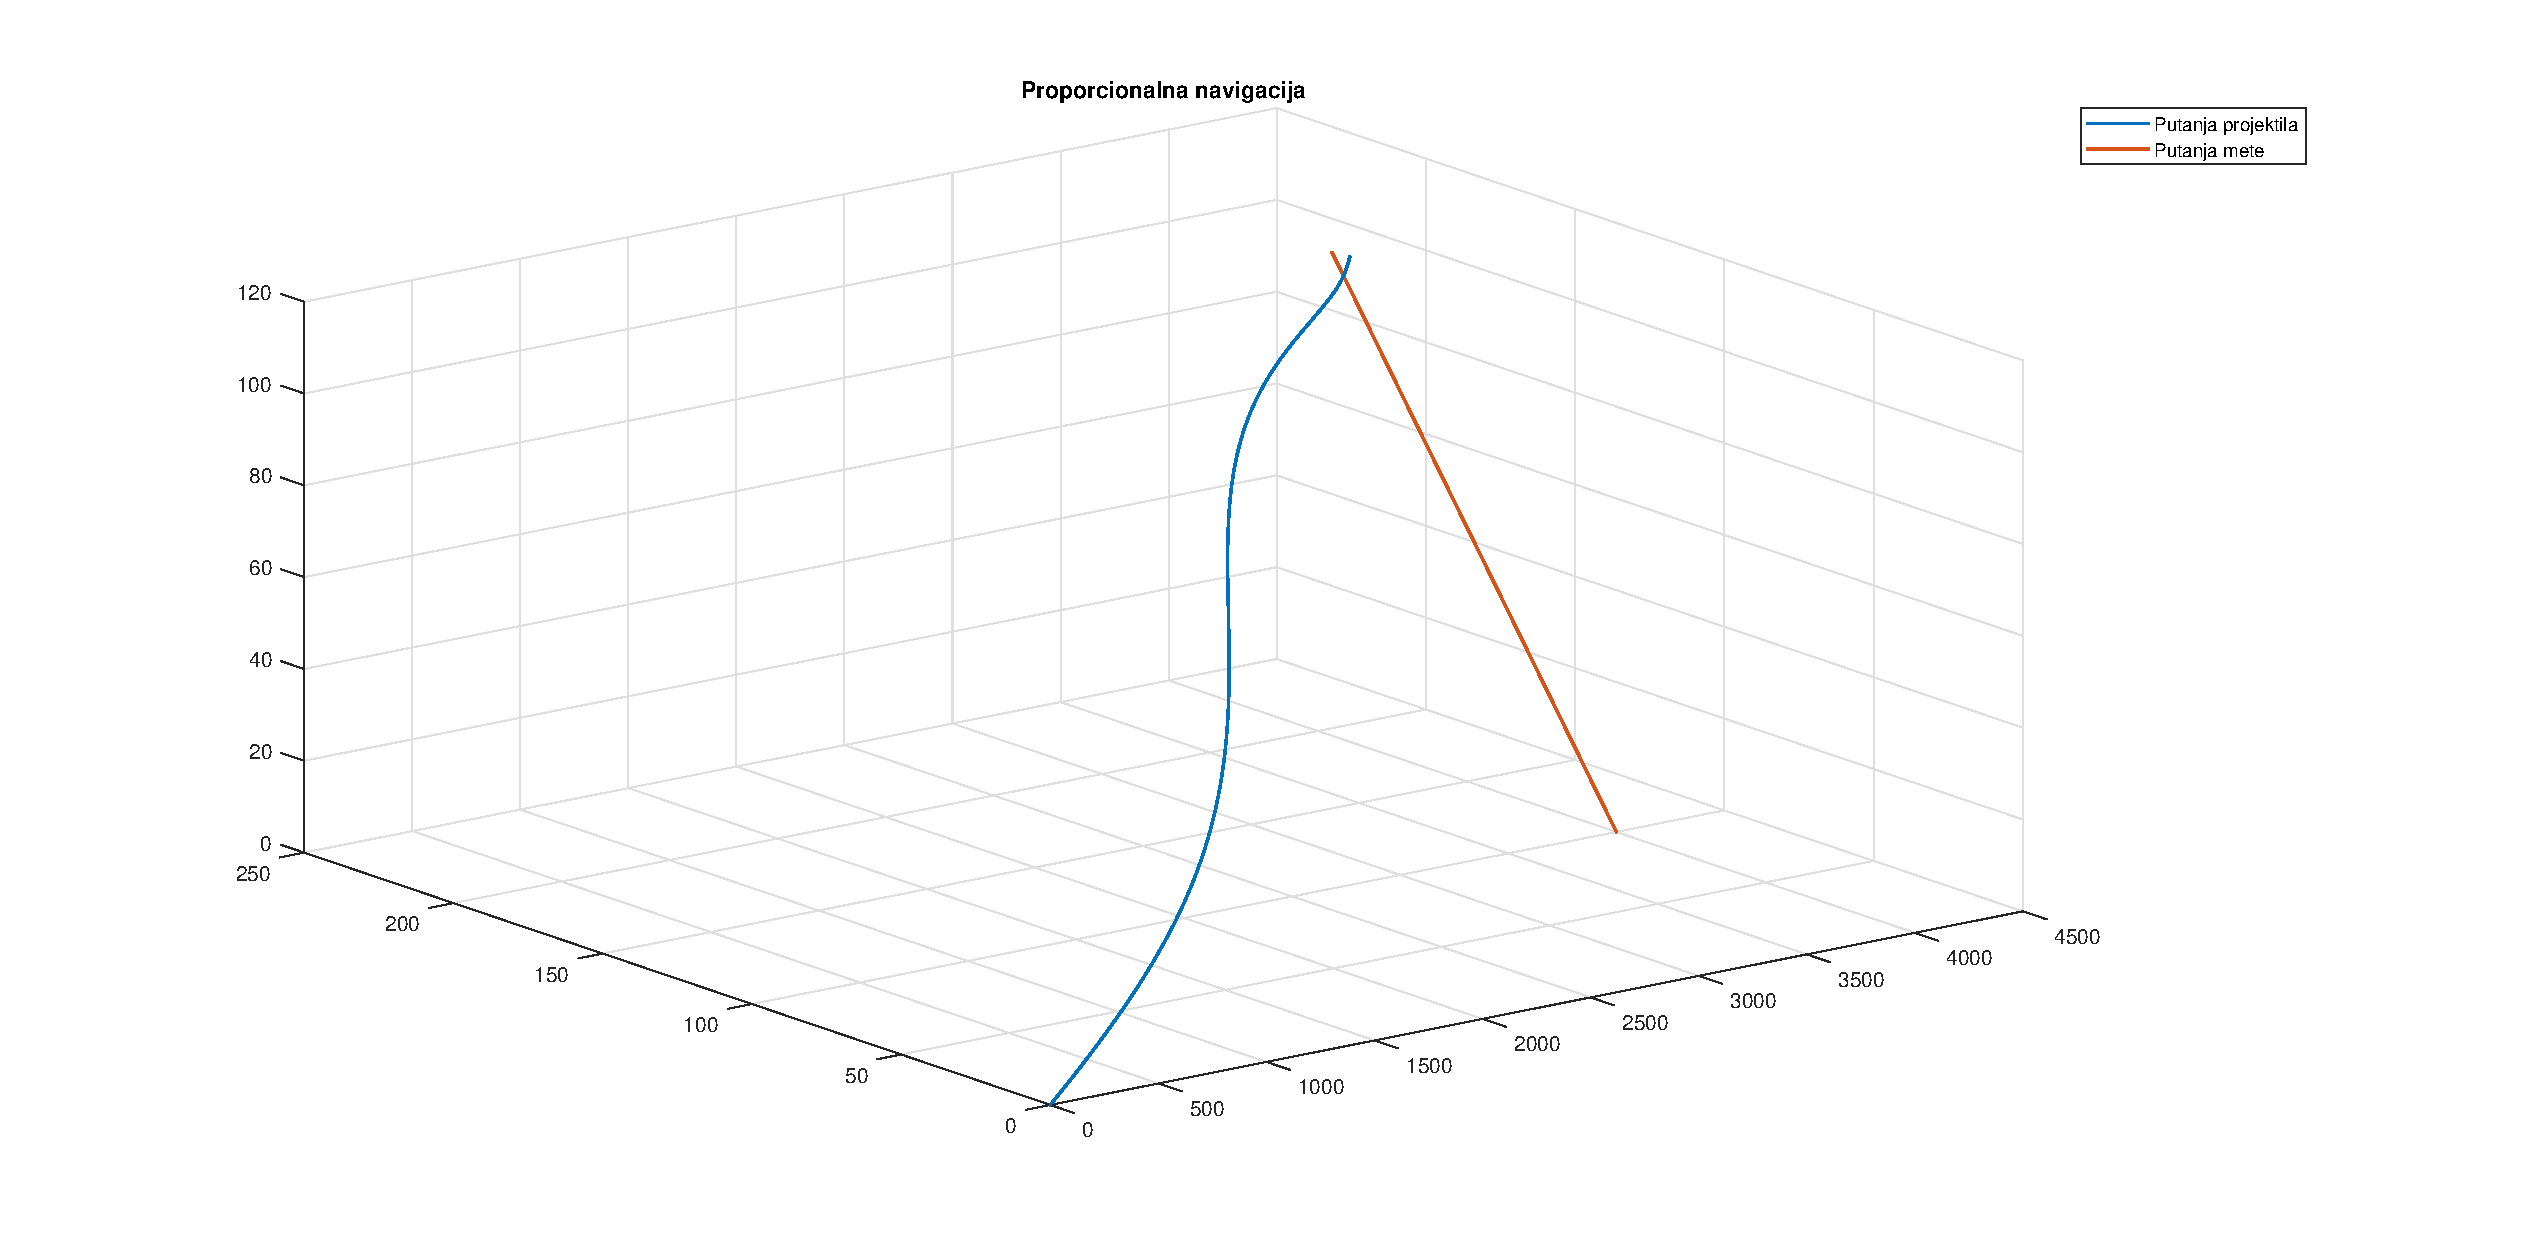
\includegraphics[scale = 0.4]{ganja2.eps}
    \caption{Putanja projektila i pokretne mete}
    \label{fig:ganja2}
\end{figure}
Vidi se da postoji neki promašaj po $y$ osi. Ovaj promašaj je usljed toga što se pri 
kraju putanje projektila javlja potreba za velikim horizontalnim ubrzanjem(priroda proporcionalne navigacije), 
a pošto je horizntalno ubrzanje neminimalne faze, ne uspijeva se pri kraju potpuno tačno orijentisati. Unatoč tome 
promašaj je jako mali i može se reći da autopilot zajedno sa sistemom vođenja uspijeva 
postići pogodak. 


